\documentclass[preprint,12pt,a4paper]{elsarticle}
\usepackage{lineno}
% \usepackage{hyperref}
\usepackage{float}
\usepackage{graphicx} % figuras
% \usepackage{subfig}
\usepackage{subfigure} % subfiguras
\usepackage{multirow} 
\usepackage{color}
\usepackage{soul}
\usepackage{cancel}

%%%%%%%%%%%%%%%%%%%%%%%%%%%%%%%%%%%%%%%%%%%%%%%%%%%%%%%%%%%%%%%%%%%%
% Init macros math

\usepackage[fleqn,tbtags]{amsmath}
\usepackage{mathtools}
\usepackage{amsthm,amssymb}
\usepackage{xstring}

\newcommand{\vect}[1]{
  \ensuremath{\mathbf{{#1}}}
}
\newcommand{\tens}[1]{
  \ensuremath{\mathbf{{#1}}}
}
\newcommand{\Matrix}[1]{
  \ensuremath{\mathbf{{#1}}}
}
\newcommand{\Vector}[1]{
  \ensuremath{\mathbf{{#1}}}
}
% Divergence
\newcommand{\Div}[1]{
  \ensuremath{div({#1})}
}
% Gradient
\newcommand\Grad[1]{grad({#1})}
\newcommand\GradS[1]{grad^s({#1})}
\newcommand\GradT[1]{grad^T({#1})}
% Partial derivative
\newcommand{\Deriv}[3][]{
  \ensuremath{\frac{\partial^{#1}{#2}}{ \partial {#3}^{#1} }}
}
% Integral
\newcommand{\Integral}[2]{
  \IfStrEqCase{#1}{
    {2}{\ensuremath{\int_{\varGamma_d}{#2}\ d\varGamma}}
    {3}{\ensuremath{\int_{\varOmega}{#2}\ d\varOmega}}
  }
}
% End macros math
%%%%%%%%%%%%%%%%%%%%%%%%%%%%%%%%%%%%%%%%%%%%%%%%%%%%%%%%%%%%%%%%%%%%


% \usepackage{algorithm,algcompatible}

\usepackage{blindtext}
\usepackage[linesnumbered,boxed]{algorithm2e}

\SetAlCapSkip{1em}

\SetKwInput{KwInput}{Input}
\SetKwInput{KwOutput}{Output}

% \usepackage[linesnumbered,ruled,vlined]{algorithm2e}
% \algnewcommand\INPUT{\item[\textbf{Input:}]}%
% \algnewcommand\OUTPUT{\item[\textbf{Output:}]}%

%%%%%%%%%%%%%%%%%%%%%%%%%%%%%%%%%%%%%%%%%%%%%%%%%%%%%%%%%%%%%%%%%%%%
% Init glossaries
\usepackage[acronym]{glossaries}

\makeglossaries

\newacronym{mpm}{MPM}{Material Point Method}
\newacronym{otm}{OTM}{Optimal Transportation Meshfree}
\newacronym{sph}{SPH}{Smoothed Particle Hydrodynamics}
\newacronym{fem}{FEM}{Finite Element Method}
\newacronym{xfem}{XFEM}{Extended Finite Element Method}
\newacronym{efgm}{EFGM}{Element-Free Galerkin Method}
\newacronym{lme}{LME}{Local Maximum-Entropy}
\newacronym{flip}{FLIP}{Fluid Implicit Particle}
\newacronym{gimp}{GIMP}{Generalized Interpolation Material Point}
\newacronym{igimp}{iGIMP}{Implicit GIMP}
\newacronym{ugimp}{uGIMP}{Uniform GIMP}
\newacronym{ddmp}{DDMP}{Dual Domain Material Point}
\newacronym{ctls}{CTLS}{Conservative Taylor Least Squares}
\newacronym{npc}{NPC}{Newmark Predictor-Corrector}
\newacronym{fe}{FE}{Forward Euler}

\newglossaryentry{domain}
{
  name=$\varOmega$,
  description={Continuum domain}
}

\newglossaryentry{contour}
{
  name=$\partial\varOmega$,
  description={Boundary of the continuum domain $\varOmega$. Also
    defined as $\Gamma$}
}

\newglossaryentry{dirichlet-boundary}
{
  name=$ \Gamma_d$,
  description={Essential or Dirichlet boundary conditions over $\partial\varOmega$}
}

\newglossaryentry{neumann-boundary}
{
  name=$ \Gamma_n$,
  description={Natural or Nemann boundary conditions over $\partial\varOmega$}
}

\newglossaryentry{a}
{
  name=$\vect{a}$,
  description={First order tensor which describes the acceleration field}
}

\newglossaryentry{v}
{
  name=$\vect{v}$,
  description={First order tensor which describes the velocity field}
}

\newglossaryentry{u}
{
  name=$\vect{u}$,
  description={First order tensor which describes the displacement field}
}

\newglossaryentry{x}
{
  name=$\vect{x}$,
  description={First order tensor which describes the global coordinates field}
}

\newglossaryentry{xi}
{
  name=$\vect{\xi}$,
  description={First order tensor which describes the local coordinates field}
}


\newglossaryentry{stress}
{
  name=$\tens{\sigma}$,
  description={Second order tensor which means the Cauchy stress tensor}
}


\newglossaryentry{strain}
{
  name=$\tens{\varepsilon}$,
  description={Second order tensor which means the Cauchy strain tensor}
}

\newglossaryentry{Constitutive}
{
  name=$\tens{D}$,
  description={Four order tensor which means the constitutive response
    of the material}
}

\newglossaryentry{LME-beta}
{
  name=$\beta$,
  description={Regularization or thermalization parameter of the
    LME$_{\beta}$ Pareto set}
}

\newglossaryentry{rho}
{
  name=$\rho$,
  description={Describes the scalar density field}
}

\newglossaryentry{fc}
{
  name=f$_c$,
  description={Compressive strenght}
}

\newglossaryentry{ft}
{
  name=f$_t$,
  description={Tensile strenght}
}

\newglossaryentry{Gf}
{
  name=G$_F$,
  description={Specific fracture energy}
}

\newglossaryentry{E}
{
  name=E,
  description={Elastic modulus}
}

\newglossaryentry{nu}
{
  name=$\nu$,
  description={Poisson ratio}
}

\newglossaryentry{Ceps}
{
  name=$C_{\epsilon}$,
  description={Normalizing constant}
}


\newglossaryentry{heps}
{
  name=$h_{\epsilon}$,
  description={Band width}
}

\newglossaryentry{Wc}
{
  name=$w_{c}$,
  description={Critical opening displacement}
}

\newglossaryentry{gamma-npc}
{
  name=$\gamma$,
  description={Time integration parameter for the \acrshort{npc} algorithm}
}

\newglossaryentry{gamma-lme}
{
  name=$\widehat{\gamma}$,
  description={Dimensionless parameter to control the value of the
    thermalization parameter $\beta$ of the \acrshort{lme} shape functions.}
}

% End glossaries
%%%%%%%%%%%%%%%%%%%%%%%%%%%%%%%%%%%%%%%%%%%%%%%%%%%%%%%%%%%%%%%%%%%%
\newcommand{\etal}{
  \textit{et al.}
}

\newcommand{\PNA}[1]{
  \textcolor{red}{{#1}}
}

\newcommand{\MMP}[1]{
  \textcolor{blue}{{#1}}
}

\newcommand{\DM}[1]{
  \textcolor{green}{{#1}}
}

%%%%%%%%%%%%%%%%%%%%%%%%%%%%%%%%%%%%%%%%%%%%%%%%%%%%%%%%%%%%%%%%%%%%

% \journal{Engineering Fracture Mechanics}
\journal{Computers and Structures}

\modulolinenumbers[5]

%%%%%%%%%%%%%%%%%%%%%%%
%% Elsevier bibliography styles
%%%%%%%%%%%%%%%%%%%%%%%
%% To change the style, put a % in front of the second line of the current style and
%% remove the % from the second line of the style you would like to use.
%%%%%%%%%%%%%%%%%%%%%%%

%% Numbered
%\bibliographystyle{model1-num-names}

%% Numbered without titles
%\bibliographystyle{model1a-num-names}

%% Harvard
%\bibliographystyle{model2-names.bst}\biboptions{authoryear}

%% Vancouver numbered
%\usepackage{numcompress}\bibliographystyle{model3-num-names}

%% Vancouver name/year
%\usepackage{numcompress}\bibliographystyle{model4-names}\biboptions{authoryear}

%% APA style
%\bibliographystyle{model5-names}\biboptions{authoryear}

%% AMA style
%\usepackage{numcompress}\bibliographystyle{model6-num-names}

%% `Elsevier LaTeX' style
\bibliographystyle{elsarticle-num}
%%%%%%%%%%%%%%%%%%%%%%%

\begin{document}

\begin{frontmatter}

\title{LME-MPM applied to quasi-brittle fracture.}

% \title{An enhanced EigenMPM }

%% Group authors per affiliation:
\author{
Miguel Molinos$^a$\footnote{Corresponding author: m.molinos@alumnos.upm.es},
Pedro Navas$^a$\footnote{Corresponding author: p.navas@upm.es},
Diego Manzanal$^a$,
and Manuel Pastor$^a$
 }
 \address{
 $^a$ ETSI Caminos, Canales y Puertos, Universidad Polit\'ectnica de Madrid.\\
 c. Prof. Aranguren 3, 28040 Madrid, Spain
}

\begin{abstract}
  The objective of this work is to introduce an alternative
  technique to address the fracture process of brittle and
  quasi-brittle materials under the \acrfull{mpm} 
  framework. With this purpose the eigensoftening algorithm, developed
  originally for the \acrfull{otm} approximation scheme, is extended
  to the \acrshort{mpm} with the aim of presenting a suitable alternative
  to the existing fracture algorithms developed for such a methodology.
  %\acrshort{mpm}. 
  The good fitting in the predictions made by the
  eigensoftening algorithm against both analytical and experimental
  results proofs the excellent performance of the method when challenging
  applications are to modeled.
\end{abstract}

\begin{keyword}
Quasi brittle fracture \sep Local-\textit{Max-Ent} approximation \sep
Material Point Method \sep Solid Dynamics
\end{keyword}

\end{frontmatter}

\linenumbers

%%%%%%%%%%%%%%%%%%%%%%%%%%%%%%%%%%%%%%%%%%%%%%%%%%%%%%%%%%%%%%%%%%%%%%%%%
\section{Introduction}
\label{sec:1}
The failure mechanisms of quasi-brittle materials and the  crack propagation have been studied from different fields such as materials science, structural engineering, earth science and petroleum engineering . The prediction of crack propagation has been approached with different numerical techniques. The \acrfull{fem} is widely used in industrial application. However, the presence of cracks is a violation of the continuity requirement of the \acrshort{fem}. To overcome this issue, numerous numerical
artifacts have been proposed with the aim of reproducing such a
complex behaviour. These techniques vary from the employment of cohesive
approaches~\cite{Barenblatt,Hilleborg_1976}, or to the gradual insertion of
cohesive elements \cite{Ortiz_1999,Pandolfi_2002,Ruiz_2000} at solid
elements boundaries. To alleviate these shortcomings of the
\acrshort{fem}, the \acrfull{xfem} in conjunction with level set
technique was introduced by Belytschko {\it et al.}
\cite{Belytschko_03} to handle arbitrary crack paths level
set. Some relevant contributions to the \acrshort{xfem} are the
modeling micro-scale crack propagation \cite{HUANG_2018}, the
introduction of a cohesive zone model \cite{NAGASHIMA_2016}, and more
recently improving it capability to predict the crack path in 3D cases
\cite{YUN_2019}.

The simulation of fracture propagation in a more accurate and effective
way can be considered as one of the ongoing goals of the development of novel spatial discretisation methods like meshfree techniques. Some
examples of it are the \acrfull{mpm}
\cite{Schreyer_2002,Chen_2002,Nairn_2003,Zhenmao_2005}, the
\acrfull{efgm} \cite{BELYTSCHKO_1995,BELYTSCHKO_2000,Zhuang_2012,Muthu_2013}, the
\acrfull{sph} \cite{Wang_2020,Wang_2019}, the \acrfull{otm} \cite{Li2010,Li_2012,Pandolfi_2013,Li_2015} or Peridynamics
\cite{HA_2011,RABCZUK_2017} among others. \\

Concerning \acrshort{mpm}, fracture has been treated numerically through two different ways. On the one hand, the ``CRAcks with Material Points (CRAMP)'' is proposed~\cite{Nairn_2003,Nairn_2006}. The basis of this methodology consist of the removal of the restriction
of the single-valued velocity field close to the crack through, at least, two sets of nodes. In this method, different labels are assigned to the material points
and nodes to distinguish if they are in the same side of the crack or
not. Under this approach, crack surface is described with line segments
in 2D and triangle patches in 3D cases. The chosen criteria for crack
propagation is based on such parameters as energy release rate
analysed by Tan \& Nairn (2002)\cite{Nairn_2002}, and the stress
intensity factor or the J-integral discussed by Guo \& Nairn
(2004)\cite{Nairn_2004}. 
On the other hand, the foundation of the second approach is the introduction of failed
material points to describe the crack evolution. In these methods, the
formation of failed points describes the nucleation of cracks, and
thereafter its propagation and branching. Consequently, the position
of the crack does not need to be explicitly stated. This fact represents
significant advantages over the ``CRAMP''. Under this approach, the
prediction of failure evolution is computed with a decohesion model,
which has been discussed by Chen {\it et al.}\cite{Zhenmao_2005} and
Schreyer {\it et al.}\cite{Schreyer_2002}. Successful simulations are provided within the framework of the fracture of brittle materials by Chen {\it et
  al.} \cite{Chen_2002,Chen_2003} and Sulsky \& Schreyer
\cite{Sulsky_2004}.\\

Similar to this approach, Schmidt {\it et al.}
\cite{Schmidt_2009} introduced the concept of eigenfracture, where
crack sets are approximated by means of eigen-deformations, which
enable the material to develop displacement jumps at no cost of local
elastic energy. Later, the eigenerosion approach to brittle fracture
was carried out by Pandolfi {\it et al.}
\cite{Pandolfi_2012,Pandolfi_2013}. In this technique, the concept of ``erosion'' of
the material point is depicted, being the material point able to remain intact or become completely failed or eroded, when no loading
capacity is bore. This method has been successfully applied to simulate high
complex phenomena such as dynamic fragmentation of metals
\cite{Li_2015}. Recently, Zhang {\it et al.}
\cite{Zhang_EE_2020} adopted the eigenerosion to resolve the dynamic
fracture of brittle materials in the \acrshort{mpm}
framework. Nonetheless, when quasi-brittle materials are simulated
though this approach, the results exhibit an overestimation of tensile
stress and strain peaks. Furthermore, since the work of Zhang {\it et al.}
\cite{Zhang_EE_2020} is made with conventional \acrshort{mpm}/\acrshort{gimp}, stress oscillations are to be faced.\\

To overcome the limitations observed in the EigenMPM
\cite{Zhang_EE_2020}, the present research proposes the eigensoftening
algorithm developed by Navas {\it et al.}
\cite{Navas_2017_ES,Navas2018a} for the \acrshort{otm} framework and
engineered for quasi-brittle materials. Inspired in the concept of the
crack band model \cite{Bazant83}, since energy dissipation is performed through the softened (or failed) volume, this methodology is able to capture the gradual rather than abrupt
dissipation of the fracture energy. Moreover, in order to mitigate stress
oscillations as well as to deal with tensile instabilities, such those that
occurs when particles crosses an element boundary, the work of Molinos~\etal~\cite{Molinos2020} is followed. The traditional \acrshort{mpm} technique is enhanced through the \acrfull{lme} approximation technique
\cite{Arroyo2006} for the spatial discretisation as well as a explicitly \acrshort{mpm} \acrfull{npc} scheme is derived for the time discretisation.\\

The paper is structured as follows. First meshfree methodology,
eigenerosion and eigensoftening algorithms are presented in Section
\ref{sec:2}. Then, both approaches are compared and verified by means of
comparisons with analytical and experimental results in Section
\ref{sec:3}. Finally, relevant conclusions are exposed in Section \ref{sec:4}.

%%%%%%%%%%%%%%%%%%%%%%%%%%%%%%%%%%%%%%%%%%%%%%%%%%%%%%%%%%%%%%%%%%%%%%%%%
\section{The meshfree methodology}
\label{sec:2}

The aim of this section is to describe and introduce some special
techniques required to face the fracture problem under the \acrshort{mpm}
framework. In consequence, this section is structured as follows: first, in
\ref{sec:2.1}, the \acrfull{npc} algorithm for the \acrshort{mpm}
will be exposed; next the \acrshort{lme} approximants are
introduced in \ref{sec:2.2} as an accurate alternative technique to
interpolate data between particles and nodes, and finally fracture
algorithms based on the eigendeformation concept are presented in
\ref{sec:2.3}.

\subsection{The \acrshort{mpm} time integration : A \acrlong{npc}  scheme}
\label{sec:2.1}
The \acrshort{mpm}~\cite{Sulsky1994} is a meshfree Lagrangian-Eulerian
method where moving material points, henceforth in this research,
particles ($\square_p$) will carry on all the physical information of the local state ($\sigma_p,
\varepsilon_p$) and a set of fixed background nodes ($\square_I$) will
be introduced to compute the balance of momentum equation. Since the
\acrshort{mpm} possesses the advantages of both Lagrangian and
Eulerian descriptions, no element distortion takes place in the
\acrshort{mpm}. Therefore, it is an appropriate and efficient method
to solve problems with moving discontinuities such as fracture evolution.\\
Without loosing generality, the \acrshort{mpm} algorithm
can be described with three main steps: (i) a variational recovery
process, where particle data is projected to the grid nodes, (ii) an
Eulerian step, where balance of momentum equation is expressed as a
nodal equilibrium equation in a FEM-like procedure, and finally
(iii) a Lagrangian advection of the particles. In the present research,
an explicit predictor-corrector time integration scheme is adopted. The
purpose of this choice is motivated due to its proved robustness and
stability for dynamic computations. In the first stage, the nodal
velocity predictor $ \vec{\tilde{v}}_I^{k+1}$ is computed through
nodal velocities $\vec{v}_I$ and accelerations $\vec{a}_I$ and evaluated
in the $k$ time step,
\begin{equation}
  \label{eq:Predictor-velocity}
  \vec{\tilde{v}}_I^{k+1} = \frac{N_{Ip}^{k} m_p (\vec{v}_p^k + (1 - \gamma)\ \Delta t\ \vec{a}_p^k)}{\tens{m}_I^{k+1}}\ .
\end{equation}
Where \gls{gamma-npc} is an user-defined parameter (typically adopted as
0.5), $\tens{m}_I$ represents the lumped mass matrix, and $N_{Ip}^{k}$ is
the nodal contribution of the shape function evaluated in the particle
coordinates $\vec{x}_p^k$. This way of computing the nodal predictor is numerically stable
as well as minimises the computational effort. Once nodal velocities are
obtained, the essential boundary conditions are imposed. After that, an
Eulerian phase is computed in the set of nodes in a
\acrshort{fem}-like way, where nodal forces $\vec{f}_{I}^{k+1}$ are
computed through the equilibrium equation. Next the nodal velocities
are corrected in a \textit{corrector} stage:
\begin{equation}
  \label{eq:Corrector-velocity}
  \vec{v}_{I}^{k+1} = \vec{v}_{I}^{pred} + \gamma\ \Delta t\
  \frac{\vec{f}_{I}^{k+1}}{\tens{m}_I^{k+1}}\ .
\end{equation}
Finally, in order to update the particles, those are advected in the Lagrangian stage as
\begin{align}
  \label{eq:Update-lagrangian-pce}
        &\vec{a}_p^{k+1} =
          \frac{N_{Ip}^k\vec{f}_{I}^{k}}{\tens{m}_I^k}\ ,\\
      &\vec{v}_p^{k+1} = \vec{v}_p^n + \Delta t\
        \frac{N_{Ip}^k\
        \vec{f}_{I}^{k}}{\tens{m}_I^k}\ ,\\
      &\vec{x}_p^{k+1} = \vec{x}_p^n + \Delta t\
         N_{Ip}^k\ \vec{v}_{I}^{k} +
        \frac{1}{2}\Delta t^2\ \frac{N_{Ip}^k\
        \vec{f}_{I}^{k}}{\tens{m}_I^k}\ .
\end{align}
The complete pseudo-algorithm it is summarised in \ref{sec:expl-pred-corr}.

\subsection{Spatial interpolation technique : \acrlong{lme} approximants}
\label{sec:2.2}
\acrfull{lme} approximation scheme was introduced by Arroyo \& Ortiz
(2006)\cite{Arroyo2006} as a bridge between finite elements and
meshfree methods. The key idea under this interpolation technique is
the interpretation of each nodal value $N_I$ as a
probability. Related with this definition, two important limits are
introduced. First the maximum-entropy (\textit{max-ent}) limit, which
ensures a \textit{unbiased statistical inference} based on the nodal
data as states the Jayne's\cite{Jaynes1957} principle of
\textit{maximum entropy}. And second the Delaunay triangulation that
warranties the \textit{least width} shape function support. To reach
a compromise between two competing objectives, a Pareto set is
defined as,
\begin{align*}
  \label{eq:LME-scheme-pareto-set}
  \text{(LME)}_{\beta} \hspace{0.15cm} &\text{For fixed} \hspace{0.15cm}
                                         \vec{x} \hspace{0.15cm} \text{minimise} \hspace{0.15cm} f_{\beta}(\vec{x}_p, N_I) \coloneqq \beta U(\vec{x}_p,N_I) - H(N_I) \\
                                       &\text{subject to}\
                                         \begin{cases}
                                           N_I \ge 0, \hspace{0.15cm} \text{I=1, ..., n} \\[1em]   
                                           \sum\limits_{I=1}^{N_n}{N_I} = 1 \\[1em]   
                                           \sum\limits_{I=1}^{N_n}{N_I \vec{x}_I} = \vec{x} \\
                                         \end{cases}
\end{align*}            
where $H(N_I)$ is the entropy of the system of nodes following the
definition given by Shannon (1948) \cite{Shannon1948}, the shape
function width is defined as $U(\vec{x}_p,N_I) \coloneqq
\sum_I N_I |\vec{x}_p - \vec{x}_I |^2$, and $\beta$ is a
regularisation o \textit{thermalization} parameter such that for
Pareto optimal solutions $\beta \in
(0,\infty)$. Notice that $\beta$ has units of $[L]^{-2}$,
therefore it can be controlled by adjusting a dimensionless
parameter\footnote{To avoid confusion with the \gls{gamma-npc} parameter of
  the \acrshort{npc}, the dimensionless parameter defined in Arroyo \&
  Ortiz \cite{Arroyo2006} as $\gamma$ will be represent by
  \gls{gamma-lme} to preserve as much as possible the original notation.},
$\widehat{\gamma}=\beta h^2$, where $h$ is defined as a
suitable measure of the nodal spacing. With the restrictions of the
Pareto set, the unique solution of the local
\textit{max-ent} problem \acrshort{lme}$_\beta$ is,
 \begin{equation}
  \label{eq:LME-p}
N_I^*(\vec{x})=\frac{\exp\left[ -\beta \; |\vec{x}-\vec{x}_I|^2 +
    \vec{\lambda}^* \cdot (\vec{x}-\vec{x}_I) \right] } {Z(\vec{x},\vec{\lambda}^*)},
\end{equation}
where $Z(\vec{x},\vec{\lambda}^*)$ is the \textit{partition function} defined as,
\begin{equation}
  \label{eq:LME-Z}
Z(\vec{x}, {\vec{\lambda}}) = \sum_{I=1}^{N_n}{ \exp \left[ -\beta \; |\vec{x}-\vec{x}_I|^2 + \vec{\lambda} \cdot (\vec{x}-\vec{x}_I)  \right]},
\end{equation}
and a Lagrange multiplier $\vec{\lambda}^*$ such minimise the function $\log
Z(\vec{x}, \vec{\lambda})$.
The traditional way to compute the optimal value of $\vec{\lambda}^*$
is through a Newton-Raphson procedure, or in more challenging
scenarios by a combination of the Newton-Raphson and the Nelder-Mead
Simplex algorithms \cite{Navas2018a}. Nonetheless, since finite
strains are not involved in the present research, Newton-Raphson is an
enough efficient method. For an uniform nodal spacing, $\beta$ can be
considered constant, thus first derivatives of the interpolation technique $\nabla
N^*_I$ can be obtained 
by evaluating the following expression
\begin{eqnarray}
  \label{eq:LME-gradp} 
\nabla N^*_I &=& -N^*_I \,  (\tens{J}^*)^{-1} \,  (\vec{x} - \vec{x}_I)
\end{eqnarray}
where $\tens{J}$ is the Hessian matrix, defined by
\begin{eqnarray}
  \label{eq:LME-J} 
  \tens{J}(\vec{x}, \vec{\lambda},\beta) &\equiv& \frac{\partial
                                                  \vec{r}}{\partial \vec{\lambda}},\\
  \label{eq:LME-r}
  \vec{r}(\vec{x},\vec{\lambda},\beta) &\equiv& \frac{\partial \log{ Z(   \vec{x},\vec{\lambda}})}{\partial \vec{\lambda}}  = \sum_I^{N_n} p_I(\vec{x},\vec{\lambda},\beta) \, (\vec{x} - \vec{x}_I).
\end{eqnarray}
An additional remark concerning the support of the interpolation
function is that, in practice, the value of $N_I$ decay exponentially following $\exp(-\beta \vec{r}
)$. In this sense,
a good practice is to truncate it under a tolerance  (typically around 10$^{-6}$) that would ensure a reasonable
range of neighbours, see \cite{Arroyo2006} for details. This tolerance
defines a limit value of the influence radius to find the neighbour
nodes of a given integration point.

\subsection{Fracture modelling approach}
\label{sec:2.3}
Within the context of \acrshort{mpm} formulation, fracture can be
modelled by failing particles according to a suitable failure
criterion. When material points are failed, they are assumed to have
null stress tensor. To reproduce this behaviour in the present
research, the eigensoftening algorithm is introduced in the 
\acrshort{mpm} framework as an alternative approach to the decohesion
model \cite{Zhenmao_2005,Schreyer_2002}. The eigensoftening concept
was originally developed by Navas {\it et al.}
(2017)\cite{Navas_2017_ES} as an extension for quasi-brittle materials
of the eigenerosion proposed by Pandolfi \& Ortiz
(2012)\cite{Pandolfi_2012} for fracture of brittle materials. The
  evaluation of both approaches \cite{Navas_2017_ES} against
  experimental measures show that the eigenerosion algorithm significantly overestimates the tensile stress and the strain peaks, meanwhile eigensoftening captures the forces and crack
patterns accurately. Furthermore,
the accuracy of this algorithm has been proven for complex fracture
patterns such as the ones obtained with fiber reinforces concrete (FRC),
\cite{Navas_2018_ES}.\\

The key idea behind the eigenerosion algorithm is the computation of the
energy-release rate attendant to the failure of material point $p$,
\begin{align}
  \label{eq:energy-release-EE}
&G_p^{k+1} = \frac{C_{\epsilon}}{m_p^{k+1}}  \sum_{x_q^{k+1} \in
  B_{\epsilon}(x_p^{k+1})} m_q W_q^{k+1}\\
  \label{eq:mass-EE}
&m_p^{k+1} =  \sum_{x_q^{k+1} \in
  B_{\epsilon}(x_p^{k+1})} m_q  
\end{align}
where $B_{\epsilon}(x_p^{k+1})$ is a $^n$dimensional sphere of radius $\epsilon$
centered at $x_p^{k+1}$. The particles which lie under this sphere are
known as the $\epsilon$-neighborhood of the material point (see
\cite{Pandolfi_2012}). This concept is conveniently sketched in
Figure \ref{fig:Failed-particles}.
%%%%%%%%%%%
\begin{figure}
  \centering
  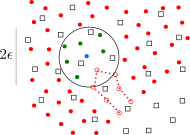
\includegraphics[width=0.5\textwidth]{Figure-Particle-failed}
  \caption{Scheme of a linear cohesive law, where the shaded area is
    $G_f$, $f_t$ is the tensile strength, and $w_c$ is the critical
    opening displacement.}
  \label{fig:Failed-particles}
\end{figure}
%%%%%%%%%%%
Other parameters are the mass of the neighborhood $m_p^{k+1}$, the
current free-energy density per unit mass  $W_q^{k+1}$ and the
normalizing constant $C_{\epsilon}$, which also defines the
  $\epsilon$-neighborhood size, being $\epsilon = C_\epsilon h$, and
  $h$ is a measure of the distance between nodes.

The failure criterion consist of considering that a material point is failed
when $G_p^{k+1}$ surpasses the critical energy release rate that
measures the material-specific energy, $G_F$. The convergence of this
approach has been analyzed by Schmidt {\it et al.}
(2009)\cite{Schmidt_2009}, who proved that $G_F$ converges to the Griffith
fracture when the discretisation size tends to zero. It is necessary to
point out that, when a material point overpass the critical energy, its
contribution to the internal forces vector is set to zero, but its
contribution to the mass matrix is preserved.\\

As can be noticed, the eigenerosion algorithm relies over an energetic
failure criterion. Because of this, unrealistic stress
concentration (higher than tensile strength) appears in quasi-brittle
materials \cite{Navas_2017_ES}. To overcome this limitation, the
aforementioned authors proposed the concept of eigensoftening to take
into account the gradual failure in quasi-brittle materials. The idea
behind this concept is inspired in the cohesive fracture. This gradual
failure criterion is plotted in Figure \ref{fig:Damage-ft-wc}, where
a linear decreasing cohesive law is presented to illustrate the
concept earlier described. In the picture, the shaded region represents
the static fracture energy per unit of area, $G_F$. Notice how a
cohesive crack appears when the maximum tensile strength, $f_t$, is
reached. Once the crack, $w_n$, reaches the value of the critical
crack opening, $w_c$, a stress-free crack is attained.
%%%%%%%%%%%
\begin{figure}
  \centering
  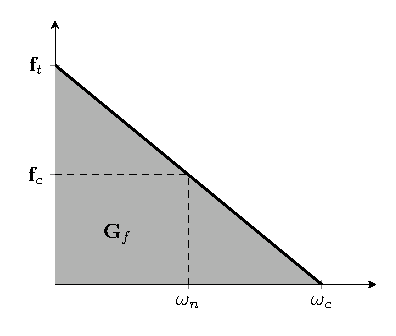
\includegraphics[width=0.5\textwidth]{Figure-Damage}
  \caption{Scheme of a linear cohesive law, where the shaded area is
    $G_f$, $f_t$ is the tensile strength, and $w_c$ is the critical
    opening displacement.}
  \label{fig:Damage-ft-wc}
\end{figure}
%%%%%%%%%%%
For the eigensoftening algorithm, a strength criterion for crack
initialization was adopted. Particularly the maximum principal stress
theory for brittle fracture was considered in \cite{Navas_2017_ES},
this allows to quantify the variation of the averaged strain energy density in the
$\epsilon$-neighborhood of the material point $\vec{x}_p^{k+1}$ as
\begin{equation}
  \label{eq:variation-averaged-strain-energy-density}
  \delta W_{\epsilon,p} = \frac{\partial G_p}{C_{\epsilon}} =
  \frac{1}{m_p} \sum_{x_q^{k+1} \in
  B_{\epsilon}(x_p^{k+1})} m_q \tens{\sigma}_{q,I} \delta \tens{\varepsilon}_q,
\end{equation}
where $\tens{\sigma}_{q,I}$ is the maximum principal stress of each
material point in the $\epsilon$-neighborhood. At this point, an \textit{effective} strain $\varepsilon_q$ is introduced in order to obtain the variation of
the local strain energy as $\delta W_q = \sigma_{q,1}
\delta\varepsilon_q$. Now, with the assumption that the effective
strain of each material point at every time step is constant in the
neighbourhood of $\vec{x}_p^{k+1}$, the equation 
\eqref{eq:variation-averaged-strain-energy-density} can be simplified
 to
\begin{equation}
  \label{eq:variation-averaged-strain-energy-density-simpli}
  \delta W_{\epsilon,p} =
  \frac{\delta \tens{\epsilon}_p}{m_p} \sum_{x_q^{k+1} \in
  B_{\epsilon}(x_p^{k+1})} m_q \tens{\sigma}_{q,I}. 
\end{equation}
Consequently, it is possible to define an equivalent critical stress at the
material point $\vec{x}_p^{k+1}$ as
\begin{equation}
  \label{eq:equivalent-critical-stress}
  \tens{\sigma}_{\epsilon,p} =
  \frac{1}{m_p} \sum_{x_q^{k+1} \in
  B_{\epsilon}(x_p^{k+1})} m_q \tens{\sigma}_{q,I}, 
\end{equation}
where $m_p$ is the total mass of the
$\epsilon$-neighborhood, defined similarly to the eigenerosion
  method (Eq.~\eqref{eq:mass-EE}). The equivalent critical stress
  leads to a definition of the   averaged strain energy in terms of the averaged
strain as $\delta W_{\epsilon,p} =
 \tens{\sigma}_{\epsilon,p}\ \delta\varepsilon_p$. The softening behaviour is
activated once $\tens{\sigma}_{\epsilon,p}^{k+1}$ surpasses the
tensile strength, $f_t$. This consists of a reduction of the internal
forces as, 
 \begin{equation}
   \label{eq:f-int-damaged}
   f^{int}_I = \sum_p (1 - \chi_p)\ \tens{\sigma}_{p}^{k+1} \cdot
   \Grad{N_{Ip}}\ \Omega_p,
 \end{equation}
where $\chi_p$ and $\Omega_p$ are respectively the damage or softening
variable and the volume for each material point $p$. $\chi_p$ is any function, taking
values between zero (an intact material) and one (completely failed
material points), that relates the crack opening and the residual strength. To calculate it, typical shapes of cohesive laws such as linear, bilinear or exponential, may be employed. For the case of a linear softening such the sketched one in the Figure \ref{fig:Damage-ft-wc}, $\chi_p$ is computed as,
 \begin{equation}
   \label{eq:damaged-variable-chi}
   1 - \chi = \frac{f_n}{f_t} = 1 - \frac{w_n}{w_c}\ \rightarrow\ \chi
   = \frac{w_n}{w_c}.
 \end{equation}
Analogous to the crack band model presented by
Bazant~\cite{Bazant83}, Navas {\it et al.} \cite{Navas_2018_ES}
\cite{Navas_2017_ES} introduced a band width parameter $h_{\epsilon}$ in order to relate the crack opening with the strain.
Concerning this parameter, a typical value between two and
four times the maximum size of the aggregates is adopted in the case of
concrete as brittle material. The effective fracture strain
$\varepsilon_{\epsilon,f}$ is defined as the difference between the strain at crack initialization,
$\varepsilon_1(\vec{x}_p^{0})$, and the current strain, $\varepsilon_1(\vec{x}_p^{k+1})$, for a material point $p$. Also,
$\varepsilon_{\epsilon,f}$ can be represented as the current crack
opening $w_n$ within the band width $h_{\epsilon}$. Therefore, 
\begin{equation}
  \label{eq:effective-fracture-strain}
  \varepsilon_{\epsilon,f} = \varepsilon_1(\vec{x}_p^{k+1}) -
  \varepsilon_1(\vec{x}_p^{0}) = \frac{w_n}{h_{\epsilon}}
\end{equation}
Introducing \eqref{eq:effective-fracture-strain} in
\eqref{eq:damaged-variable-chi}, the damage variable can be computed
as,
\begin{equation}
  \label{eq:damage-variable-chi-II}
\chi = \frac{\varepsilon_{\epsilon,f}\ h_{\epsilon}}{w_c}.  
\end{equation}
The function of $\chi$ presented in \eqref{eq:damage-variable-chi-II}
represents a linear softening behaviour. For a general case, the
damage variable can be expressed in terms of the following variables,
\begin{equation}
  \label{eq:damage-variable-chi-III}
  \chi = \chi(\varepsilon_{\epsilon,f}, h_{\epsilon}, f_t, w_c, G_f)
\end{equation}
Implementation details can be consulted in \ref{sec:eigens-algor-1}.

\subsection{$\epsilon$-neighbourhood reconstruction : A node-linked method}
\label{sec:epsil-neighb-reconst}
The construction of the $\epsilon$-neighbourhood is a major issue of the proposed methodology. Since this operation could be extremely demanding, optimal
numerical implementation should be employed. In opposite with the Cell-linked
method proposed by Allen \& Tildesley \cite{Allen_et_al_1989} where
the definition of a numerical tolerance is required for auxiliar
algorithms like Crossing Number \cite{Shimrat_1962} or Correct
Even-Odd \cite{Galetzka_et_al_2017}, the proposed methodology adopted herein is linked to the shape function neighbourhood. In order to avoid the aforementioned error prone
techniques, we endeavour to exploit the meshfree benefits of
the \acrshort{lme} approximants to introduce a node-linked method. Due
to the global support of this interpolation technique, the classical
interpretation of the \acrshort{fem} element typically adopted in
\acrshort{mpm} simulations is not required anymore. Instead, a linked
list with the surrounding nodes for each node is defined at the initial
time. Also, each particle has to be associated with the
closest node instead of with the belonging element as heretofore has been
done.
Now lets define the concept of a particle \textit{tributary nodes} as the
list of nodes close to it among which the information transfers
occurs. Once the closest nodes are defined, the particle
possesses automatically a list of \textit{tributary nodes}. This has two
immediate benefits: the first one is that shape functions with global
support as \acrshort{lme} are easier to be implemented,
and the second one is the increase of the efficiency of the $\epsilon$-neighbourhood
reconstruction. Regarding this last benefit, since the current
particle has a \textit{tributary nodes} list assigned to it, and
consequently each node has a linked list with a set of
\textit{tributary particles}\footnote{Notice that the list of the
  particles close to each node is unique for each node and is updated
  in each time step.} close to it, it is possible to define efficiently a
search list with those particles close to the current particle.
In the end, particles out of the area of influence, Figure
\ref{fig:Failed-particles}, are pop out of the final
$\epsilon$-neighbourhood. A final remark about this new approach is
its ability to reconstruct easily a search list with the support of
the initial connectivity of the mesh. It provides a suitable basis for
an easy implementation of other interpolation techniques with minimum
coding effort. A detailed explanation of the proposed algorithm can be
found in \ref{sec:node-linked-method-1}.
%%%%%%%%%%%%%%%%%%%%%%%%%%%%%%%%%%%%%%%%%%%%%%%%%%%%%%%%%%%%%%%%%%%%%%%%%

\section{Cases of study and discussion}
\label{sec:3}

The proposed approach to overcome the two main shortcomings of
EighenMPM \cite{Zhang_EE_2020} has been evaluated with ``three
benchmark tests''.
The first one deals with the presence of stress
instabilities provoked by the spatial discretisation, appearing even when the \acrshort{gimp} shape functions are employed. To overcome it, \acrshort{lme}
approximants are introduced as an alternative to the existing interpolation techniques. Its
performance in mitigating spurious stress oscillations under the \acrshort{mpm}~\cite{Wobbes2020,Molinos2020} framework helps to enhance
notoriously the quality of the results as it is observed in Section
\ref{sec:3.1}, where both interpolation techniques
are compared by carrying out an eigenerosion simulation. The second
limitation is concerned to its inability to simulate properly quasi-brittle
fracture \cite{Navas_2018_ES}. It can be solved through the
eigensoftening algorithm described in Section \ref{sec:2.3}. A proof
of it is exposed in Sections \ref{sec:3.2} and \ref{sec:3.3}, where experimental results
are compared with numerical ones, being the eigensoftening technique the one employed in this research for the
computations. In the first case comparing with a semicircular bending
test and in the second case with a drop-weight impact test.


\subsection{Edge-cracked square panel in mode I}
\label{sec:3.1}
The aim of the problem presented hereinafter is to assess the
capability of the \acrshort{lme} approximants to improve the result
\textit{versus} the standard linear interpolation and \acrshort{ugimp}
\cite{Bardenhagen2004}. The application
consists of a square plate of size $H = 1\ [L] $ containing an initial edge
crack of length $0.25 \cdot H$ loaded in a pure mode I by displacement
control on the outer flanks of the plate (See Figure
\ref{fig:geometry-cracked-panel-mode-I} for details). 
%%%%%%%%%%%%%%%%%%%%%%%%%%%%%%%%%%%%%%%%%%%%%%%%%%
\begin{figure}
  \centering
  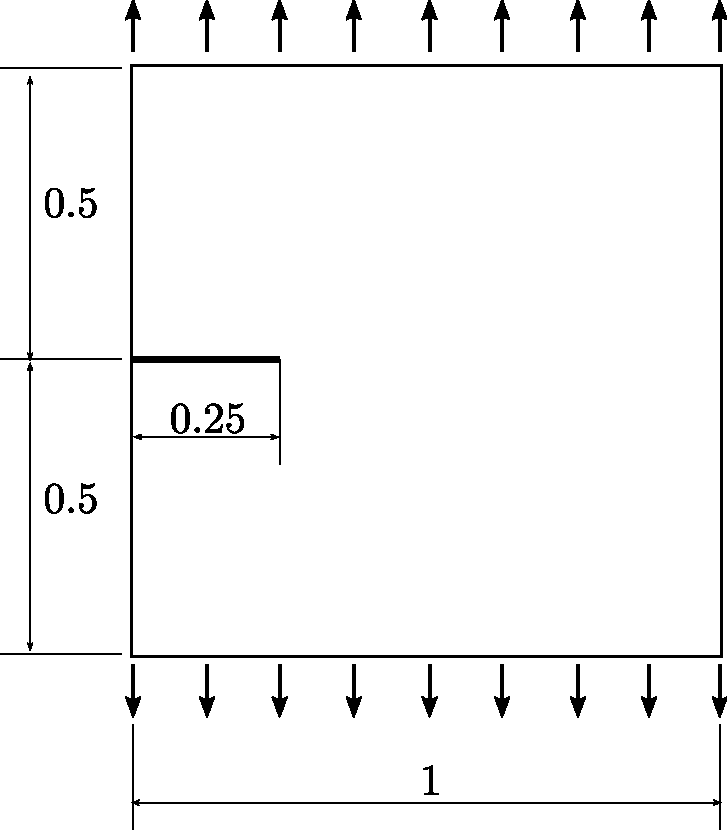
\includegraphics[width=0.4\textwidth]{Figure-Mode_I}
  \caption{Geometry and boundary condition of the drop-weight impact test.}
  \label{fig:geometry-cracked-panel-mode-I}
\end{figure}
%%%%%%%%%%%%%%%%%%%%%%%%%%%%%%%%%%%%%%%%%%%%%%%%%%
The constitutive model considered in the numerical experiment is a
linear-elastic Hookean material, whose Young's modulus \gls{E} = 1.06
$[M] [L]^{-1} [T]^{-2}$, the Poisson's ratio \gls{nu} = 0.333, and
critical energy-release rate \gls{Gf} = 0.0001 $[L]^{2} [T]^{-2}$. The absence of units is due to the current
simulation will not be tested against experimental results, where
scale factor is relevant, but will be validated against an analytical
solution provided by Pandolfi \& Ortiz \cite{Pandolfi_2012}. In
\acrshort{mpm}, two different discretisation are required. On one
hand, a cartesian grid of nodes is considered with a nodal spacing
value of 0.025 $[L]$. On the other hand, the plate will be modeled with a
initial layout of four particles per element and occupying the Gauss
quadrature positions.\\

Figure \ref{fig:Reactions-cracked-panel-mode-I} clearly shows that the
\acrshort{lme}$_{\gamma = 3.5}$ solution has a reaction peak value of 0.03 $[M] [L]
[T]^{-2}$ for a imposed displacement 0.015 $[L]$ which agrees with the
analytical solution \cite{Pandolfi_2012}. It also shows the presence
of wiggles in the reaction-displacements curve, in both loading and
post-failure stages, when linear interpolation technique is used. In
contrast, \acrshort{lme} simulation does not exhibit these spurious
oscillations and remains linear until the failure. About the strength,
linear interpolation produces stiffer results than \acrshort{lme}. This can be attributed to imprecision in the
stress field due to grid-crossing phenomena. Alternative to
  \acrshort{lme}, \acrshort{ugimp} shape
functions can be employed to mitigate grid-crossing instabilities.
Figure \ref{fig:Reactions-cracked-panel-mode-I} supports this fact since it
does not exhibit instabilities when particles cross element borders meanwhile these instabilities are found with linear interpolation. Unfortunately, the extended support of this
kind of shape function interfere with nodes in both sides of the notch,
producing an undesired ``tie-effect''. This involves in a violation of
the free border boundary condition in the notch. Possible solutions to this effect
are the suppression of the elements in the notch, within a CRAMP-like
method where two pairs of nodes are employed, or reducing the mesh size. With \acrshort{lme}
approximants these artefacts are not required since it is possible to control the support
of the shape function reducing the grid-crossing and avoiding the
``tie-effect'' in the notch at the same time.\\
%%%%%%%%%%%%%%%%%%%%%%%%%%%%%%%%%%%%%%%%%%%%%%%%%%%%%%
\begin{figure}
  \centering
  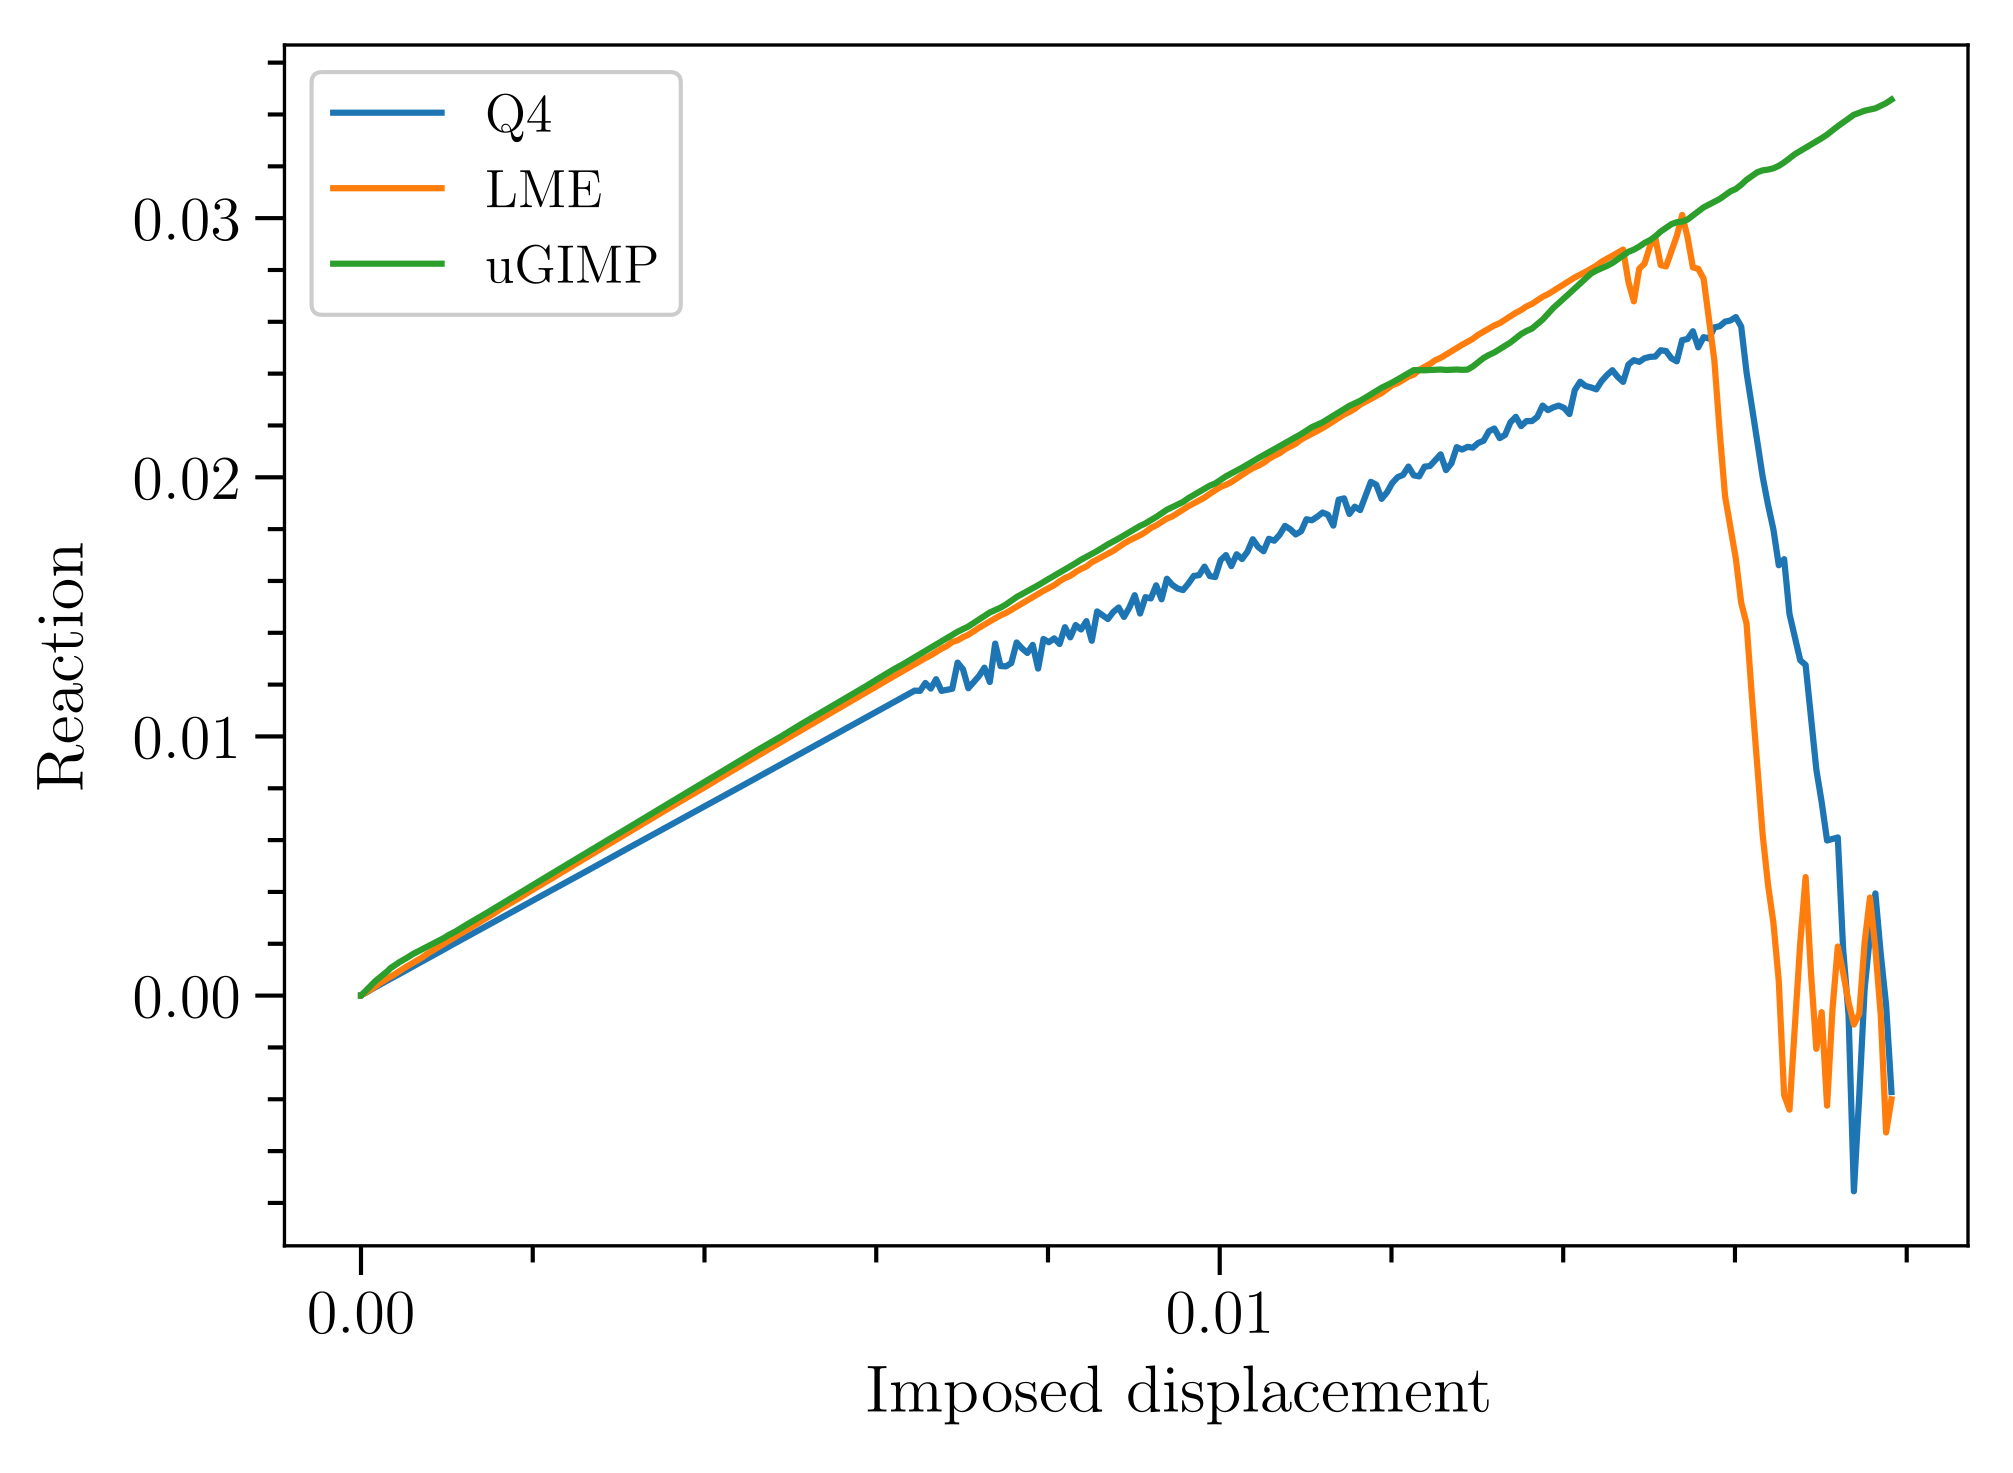
\includegraphics[width=0.8\textwidth]{Figure-Reactions-Mode-I}
  \caption{Evolution of the reaction forces plotted \textit{versus}
    the imposed displacement for linear interpolation technique and
    the \acrshort{lme} approximants.}
  \label{fig:Reactions-cracked-panel-mode-I}
\end{figure}
%%%%%%%%%%%%%%%%%%%%%%%%%%%%%%%%%%%%%%%%%%%%%%%%%%%%%%
Additionally, Figure \ref{fig:Stress-cracked-panel-mode-I}
remark clearly the difference between linear interpolation and
\acrshort{lme}, since numerical instability becomes rather significant
when particles crosses the boundary of the element in the linear
case, which is observed at 60 seconds. Although, apparently, the
differences in the obtained peaks are not extremely significant, it
can be owing to the aforementioned hookean material
employed~\cite{Zhang_EE_2020}. When more sophisticated constitutive
models will be employed, severe inaccuracies may appear in the
stress field that could affect dramatically to the final 
result. Focusing on the post failure behavior, it can be seen how
\acrshort{lme} produces soft stress field evolution even after
breaking. 
%%%%%%%%%%%%%%%%%%%%%%%%%%%%%%%%%%%%%%%%%%%%%%%%%%%%%%
\begin{figure}
\centering
\subfigure[t = 25]{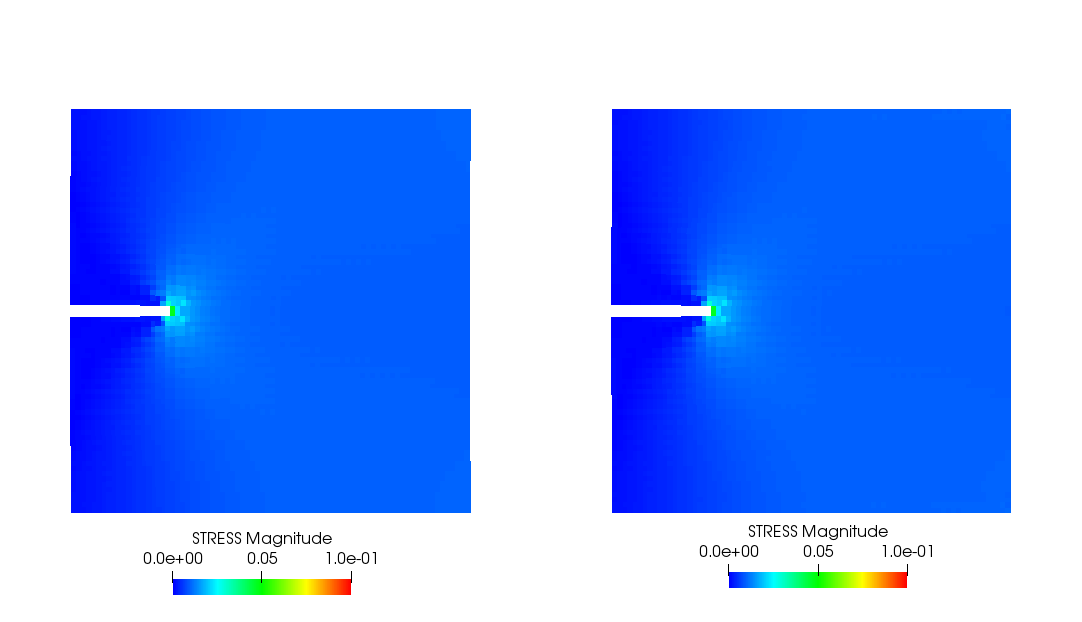
\includegraphics[width=0.73\textwidth]{./Figure-Stress-0100-mode-I.png}}
\subfigure[t = 60]{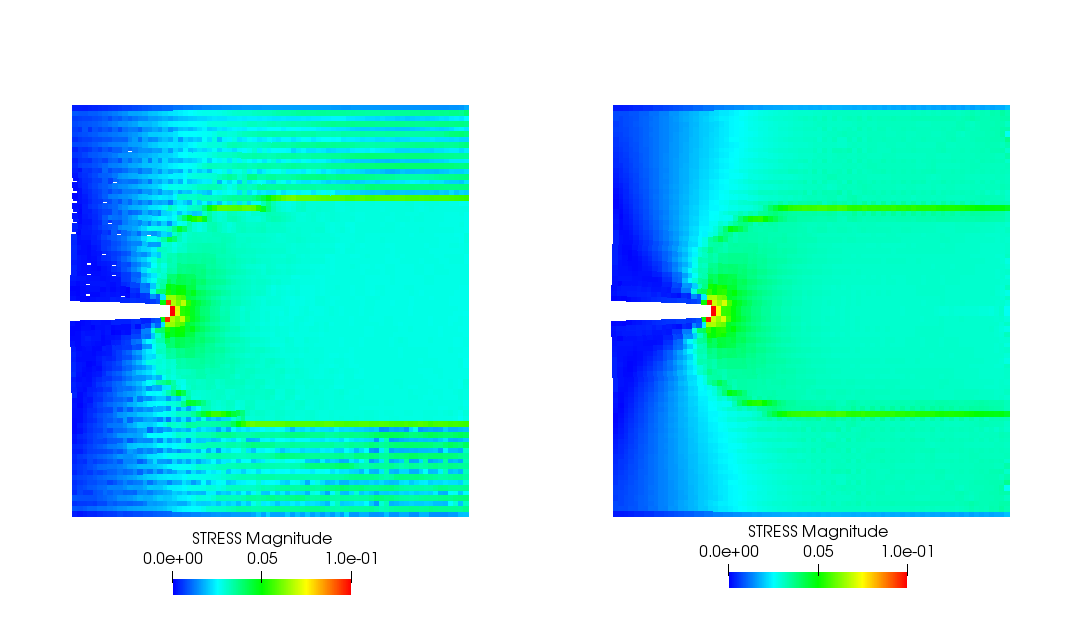
\includegraphics[width=0.73\textwidth]{./Figure-Stress-0250-mode-I.png}}
\subfigure[t = 100]{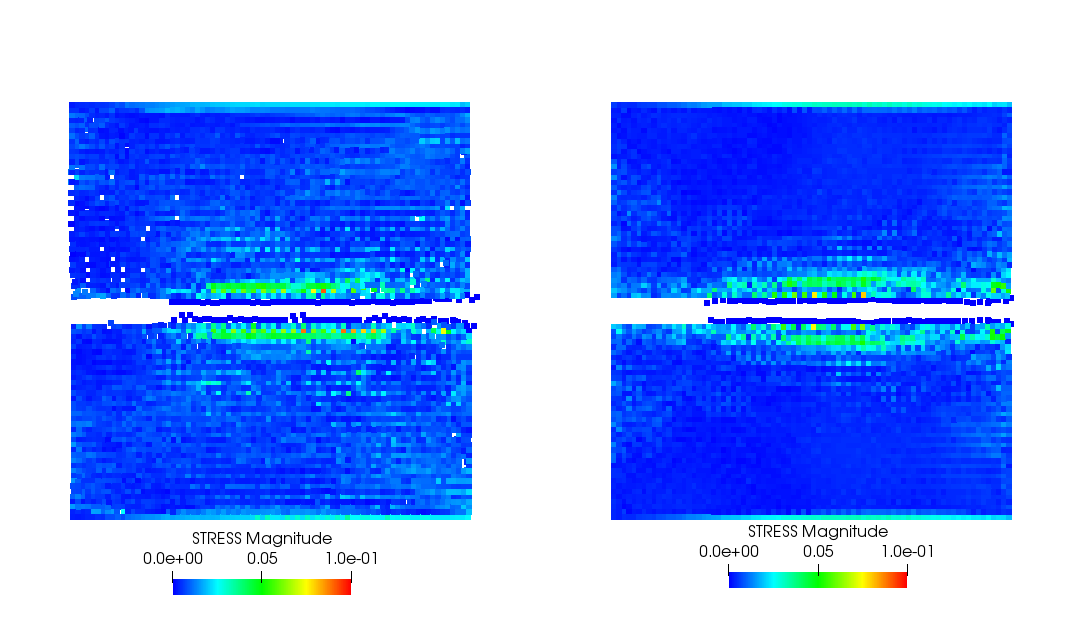
\includegraphics[width=0.73\textwidth]{./Figure-Stress-0398-mode-I.png}}
\caption{Evolution of the stress tensor magnitude for linear
  interpolation (pictures in the left side), and \acrshort{lme}
  (pictures in the right side). Both simulations performed with an
  eigenerosion algorithm.}
\label{fig:Stress-cracked-panel-mode-I}
\end{figure}
%%%%%%%%%%%%%%%%%%%%%%%%%%%%%%%%%%%%%%%%%%%%%%%%%%%%%%
An important consideration regarding the presence of oscillations once
both parts of the panel are separated is observed in Figure
\ref{fig:Reactions-cracked-panel-mode-I}. These phenomena should not be
attributed to the eigenerosion algorithm since the fracture process is
over. They are due to the dynamic nature of the solver: once the
energy is released dinamically by the crack, the waves propagate
along the domain.


\subsection{Semicircular bending test}
\label{sec:3.2}

The second application to be considered analyses the bending behavior of semicircular specimens of Johnstone rocks, text which were experimentally carried out by Lim {\it et
  al.} \cite{LIM_1993} and numerically reproduced by Wang {\it et
  al.}\cite{Wang_2020} under \acrshort{sph} framework within an
implicit algorithm. The aim of the test is to examine the predictive
capability of the eigensoftening algorithm under different kind of
mixed-mode loading conditions. This capability was assessed previously within a
\acrshort{otm} implementation \cite{Navas_2018_ES}.

The geometry and boundary conditions are sketched in Figure 
\ref{fig:geometry-Semicircular-bending-test}. The experiment consist of loading
semicircular specimens with a radius of 47.5 mm and a thickness of
20 mm, supported by two rollers at a span of 47.5 mm, by
another roller on its top mid-span. Notches with a length of 16.6 mm are
created with the different notch angles of 0$^{\circ}$, 30$^{\circ}$ and 60$^{\circ}$ with respect
to the vertical axis in order to investigate the influence of the
notch angle on the peak load \ref{fig:plot-Angle-Forces-test}.
%%%%%%%%%%%%%%%%%%%%%%%%%%%%%%%%%%%%%%%%%%%%%%%%%%%
\begin{figure}
  \centering
  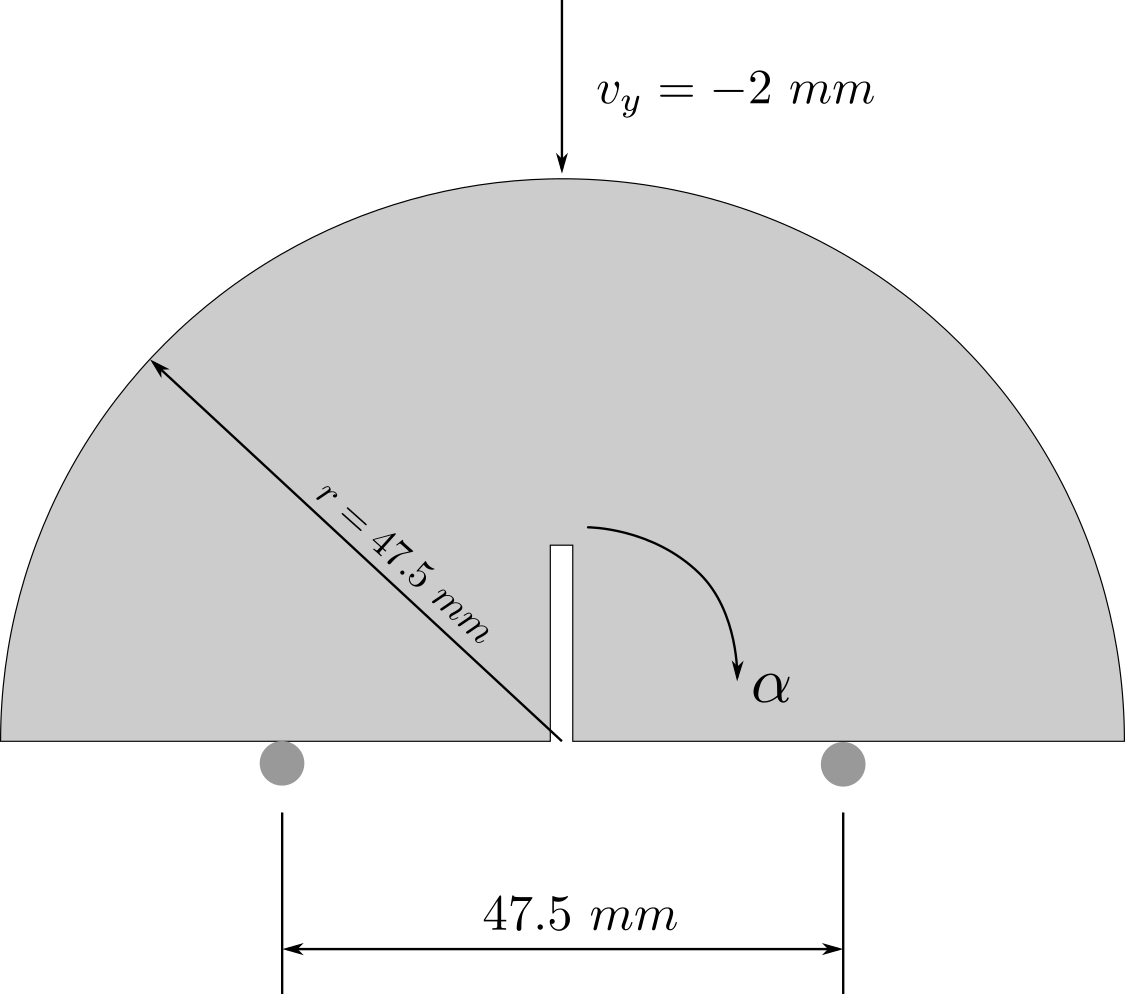
\includegraphics[width=0.6\textwidth]{./Figure-Semicircular-bending-test}
  \caption{Geometry and boundary condition of the semicircular bending
    test.}
  \label{fig:geometry-Semicircular-bending-test}
\end{figure}
%%%%%%%%%%%%%%%%%%%%%%%%%%%%%%%%%%%%%%%%%%%%%%%%%%%
The material properties of Johnstone rock are listed in Table \ref{tab:Johnstone-properties}.
%%%%%%%%%%%%%%%%%%%%%%%%%%%%%%%%%%%%%%%%%%%%%%%%%
\begin{table}
  \centering
  \begin{tabular}[]{l l}
    \hline
    Young's modulus (\gls{E})   & 0.4\ $GPa$       \\
    Poisson ratio (\gls{nu})    & 0.25           \\
    Density (\gls{rho})         & 1.54\ $g/cm^3$ \\
    Tensile strength (\gls{ft}) & 0.6\ $MPa$       \\
    Critical opening displacement (\gls{Wc}) & 0.015\ $mm$ \\
    \hline
  \end{tabular}
  \caption[Mechanical properties of Johnstone. ]{Material properties of Johnstone.}
  \label{tab:Johnstone-properties}
\end{table}
%%%%%%%%%%%%%%%%%%%%%%%%%%%%%%%%%%%%%%%%%%%%%%%%%
In the tests, particles were uniformly distributed with an almost
constant separation of 1 mm between them, resulting in a total number of 4672
\acrshort{mpm} particles for generating the specimen. Additionally, a
regular cartesian background grid of 1917 nodes with 1.5 mm of nodal distance
was generated. The velocity of the top boundary particles is $v_y = − 2 mm/s$, 
whereas the velocity of the bottom boundary particles is $v_y$ = 0 mm/s.
To reduce dynamic effects due to a sudden loading, a soft loading ramp has been employed as a loading curve. 
Finally, the model was calibrated with a regularization parameter \gls{Ceps} = 1.7 and a
bandwidth value \gls{heps} = 15.

Figure \ref{fig:Figure-Angle-Forces-test-damage-pattern} shows the
comparison of mixed-mode fracture envelope between experiments and
\acrshort{mpm} simulations for different notch inclination angles
$\alpha$ = 0$^{\circ}$, 30$^{\circ}$ and 60$^{\circ}$. The final
fracture pattern is a vertical straight line when $\alpha$ = 0$^{\circ}$  (pure mode I). 
When $\alpha > 0^{\circ}$, the sample is
subjected to a mixed-mode pattern. For the cases of 0$^{\circ}$ and 30$^{\circ}$, cracks
initiate from the notch tip and then propagate towards upper loading
point. Experiments show that a few cracks tend to initiate behind
notch tip when the notch angle is beyond 50$^{\circ}$. Figure
\ref{fig:Figure-Angle-Forces-test-damage-pattern} demonstrates that
eigensoftening, combined with \acrshort{mpm}, is able to reproduce this
behavior. Therefore, the simulation results predict successfully the
fracture envelope in experiments and demonstrate the capability of
the eigensoftening-\acrshort{mpm} model for capturing the fracture
development under various complex loading conditions. 
%%%%%%%%%%%%%%%%%%%%%%%%%%%%%%%%%%%%%%%%%%%%%%%%%%%%%%%
\begin{figure}
\centering
\subfigure[$\alpha$ = 0]{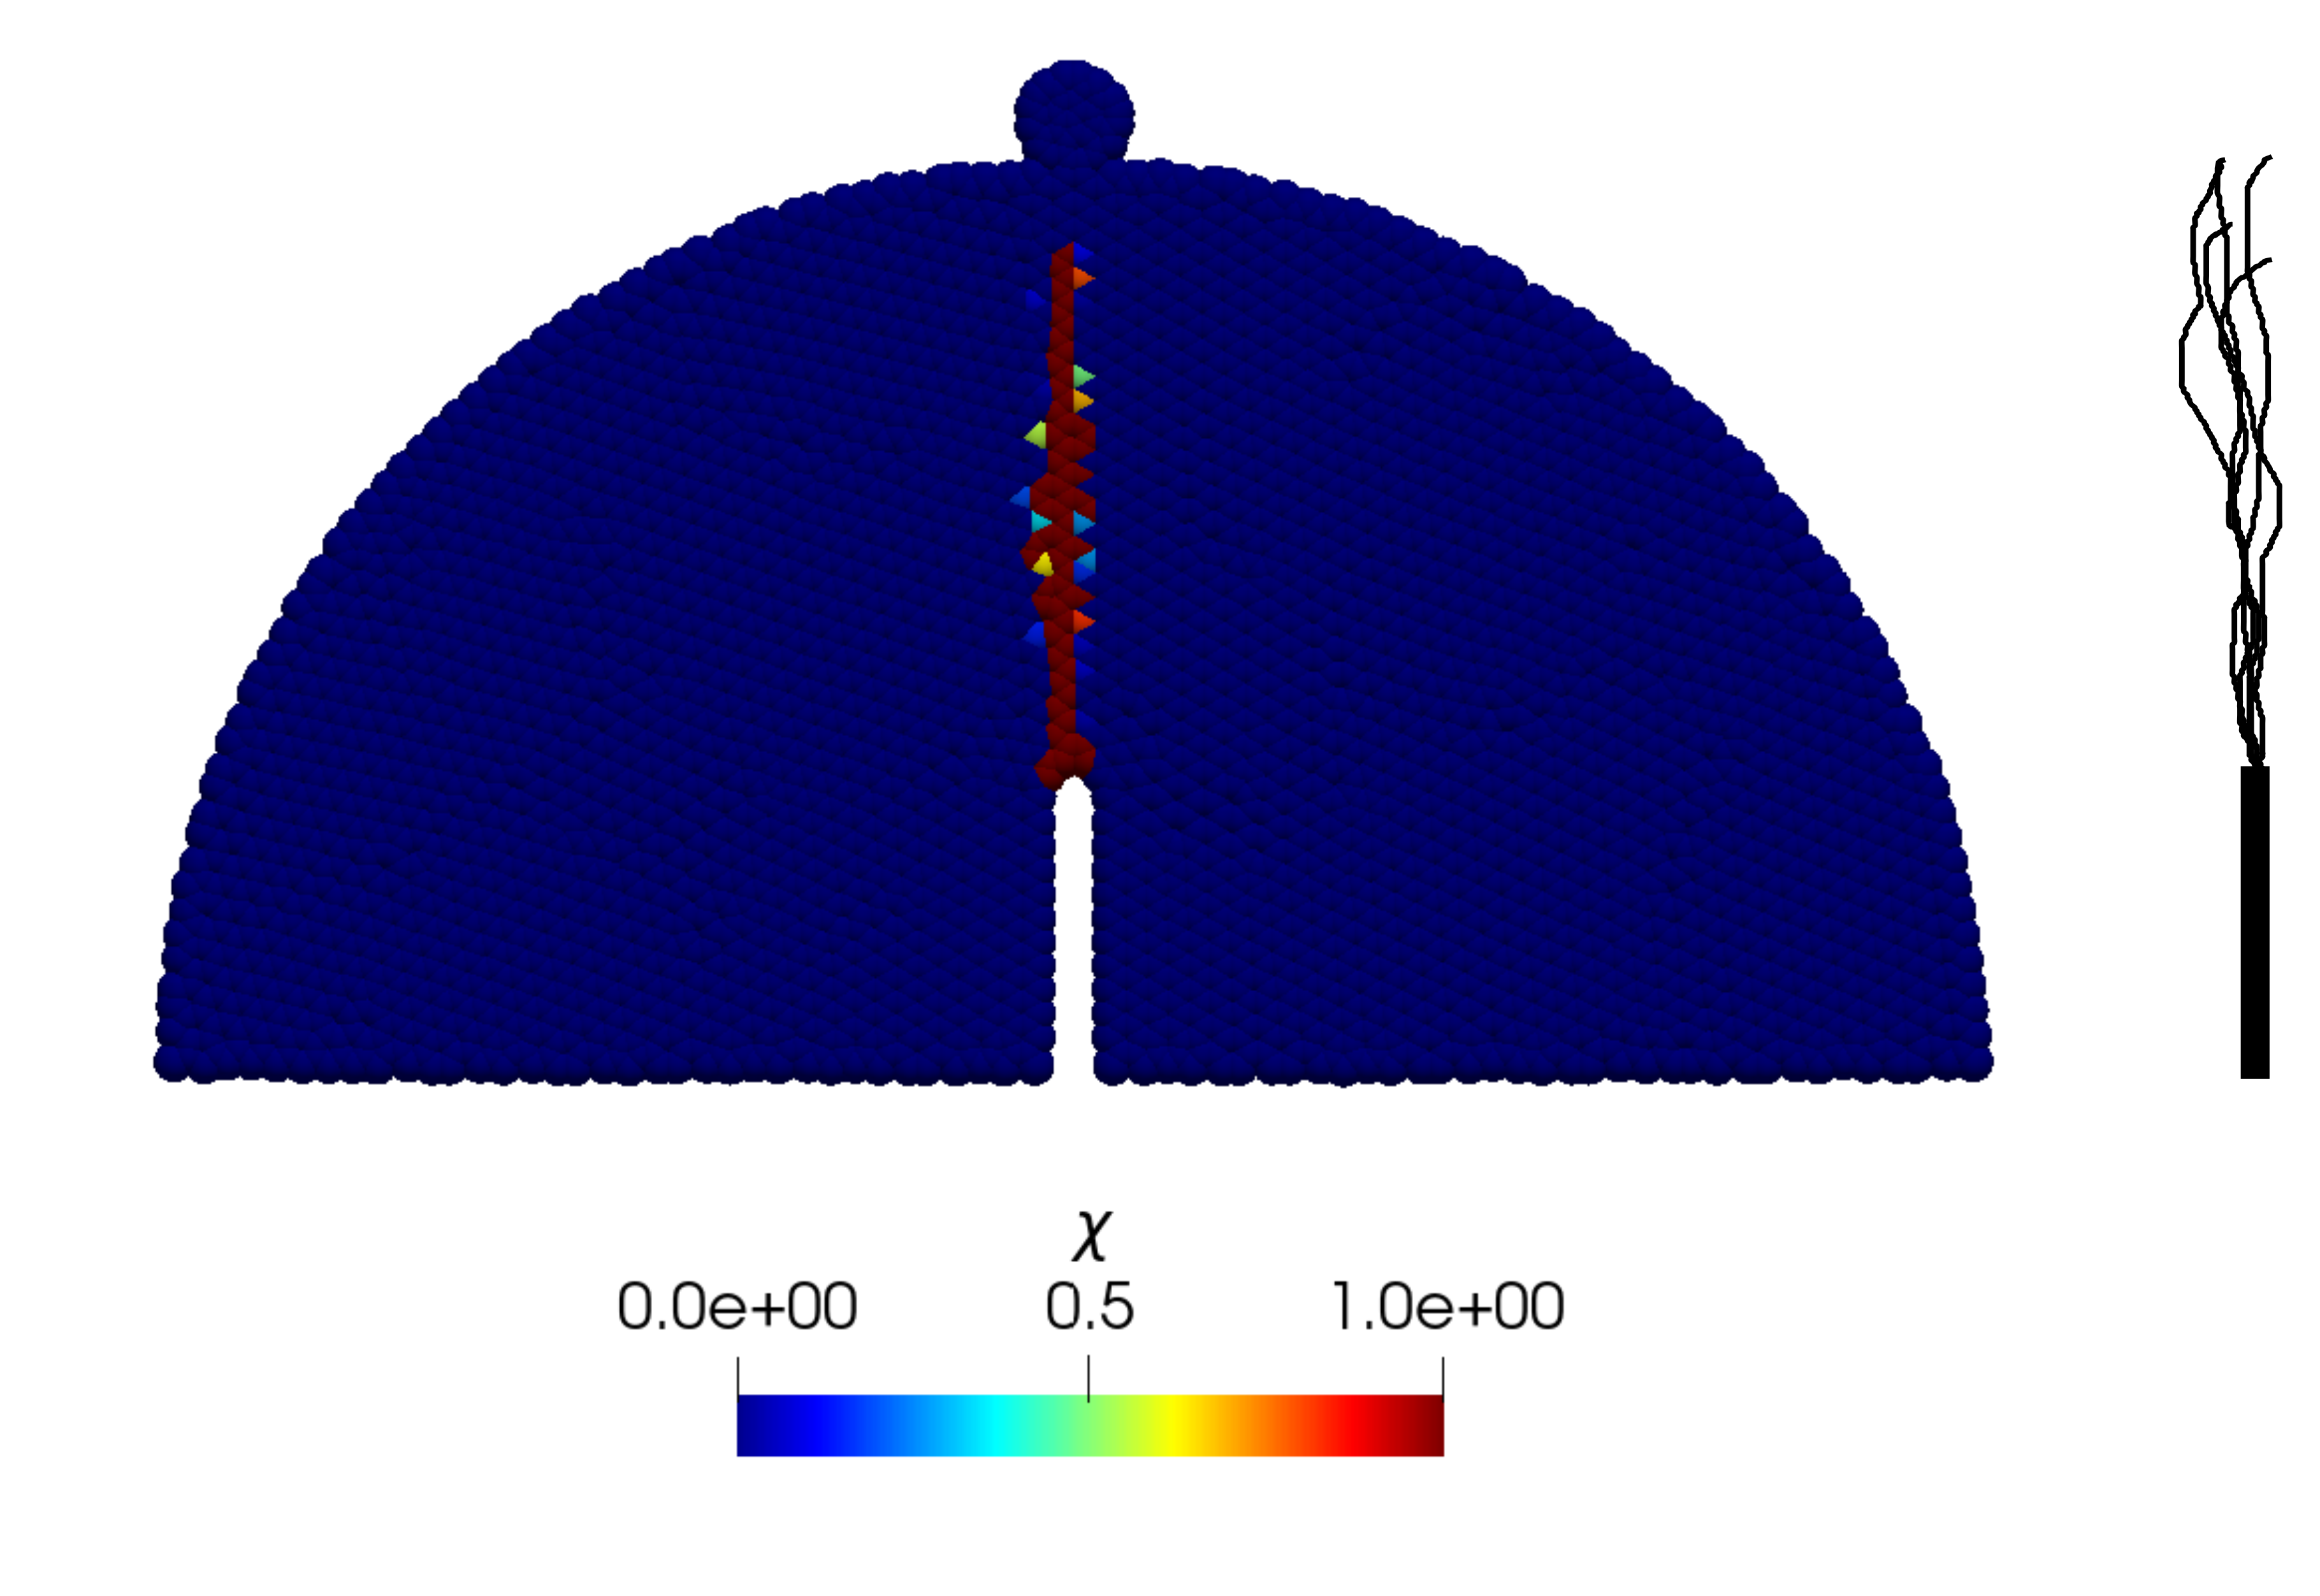
\includegraphics[width=0.49\textwidth]{./Figure-Angle-Forces-test-0-damage-pattern.png}}
\subfigure[$\alpha$ = 30]{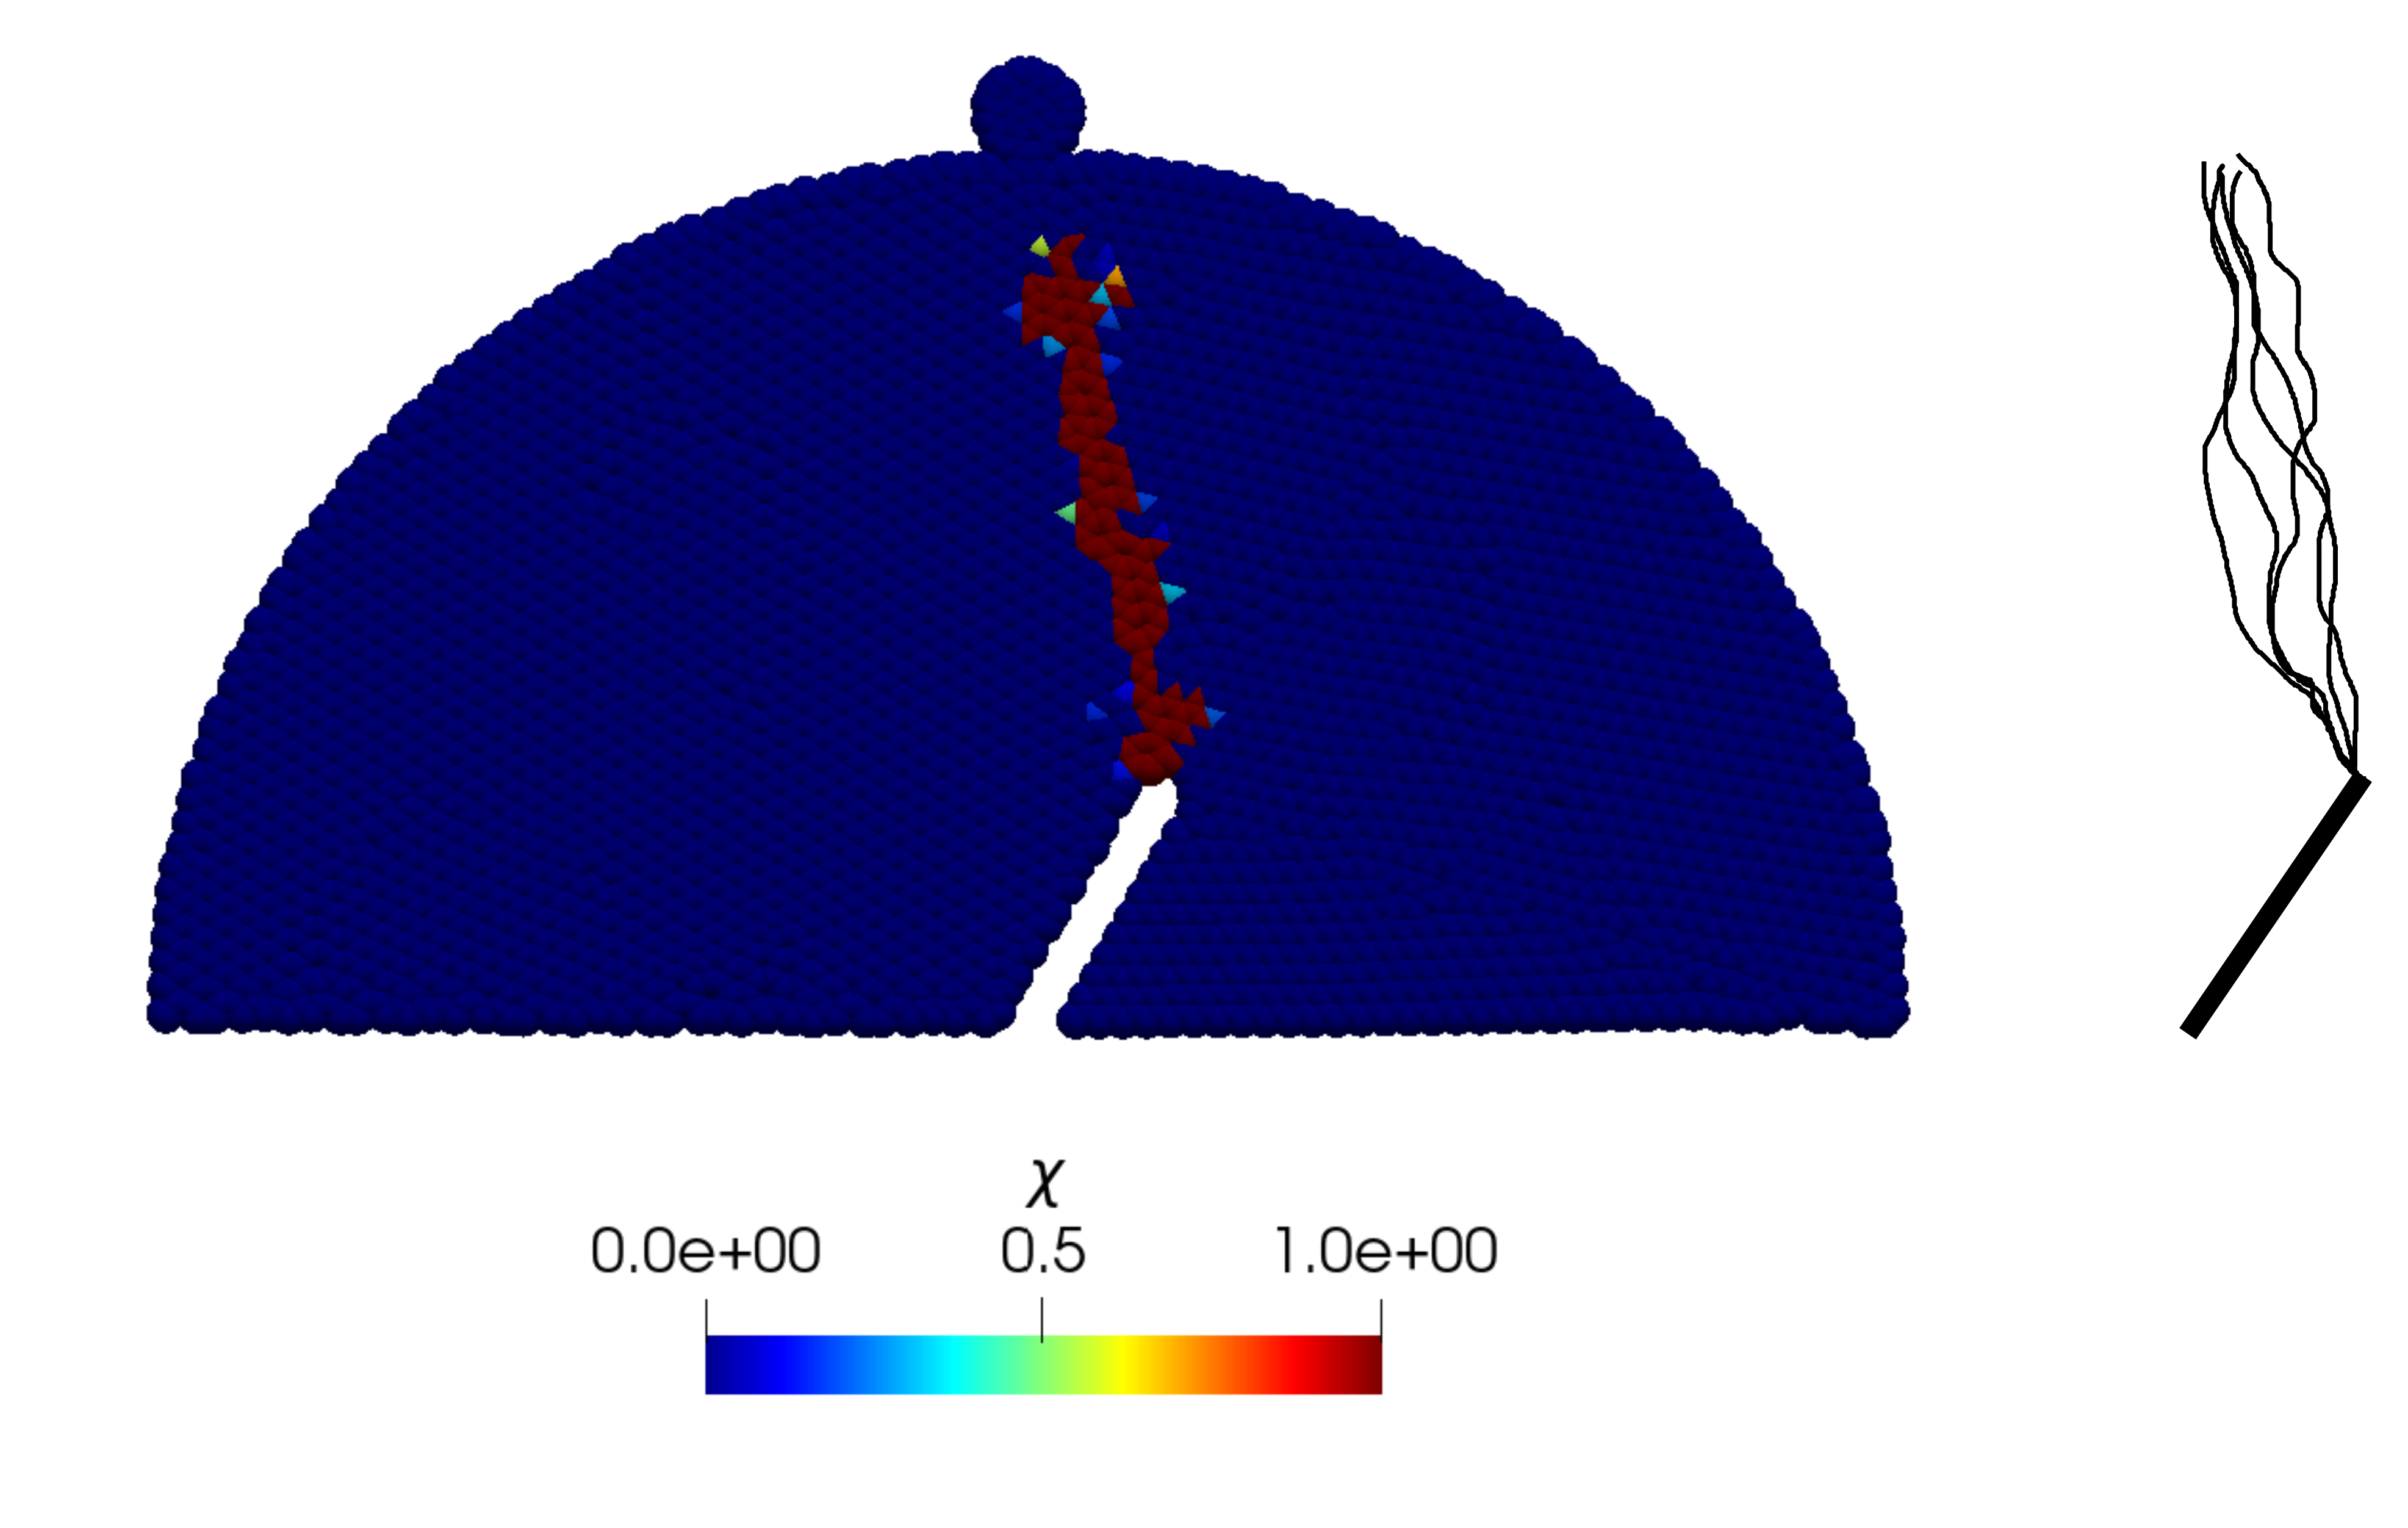
\includegraphics[width=0.49\textwidth]{./Figure-Angle-Forces-test-30-damage-pattern.png}}
\subfigure[$\alpha$ = 60]{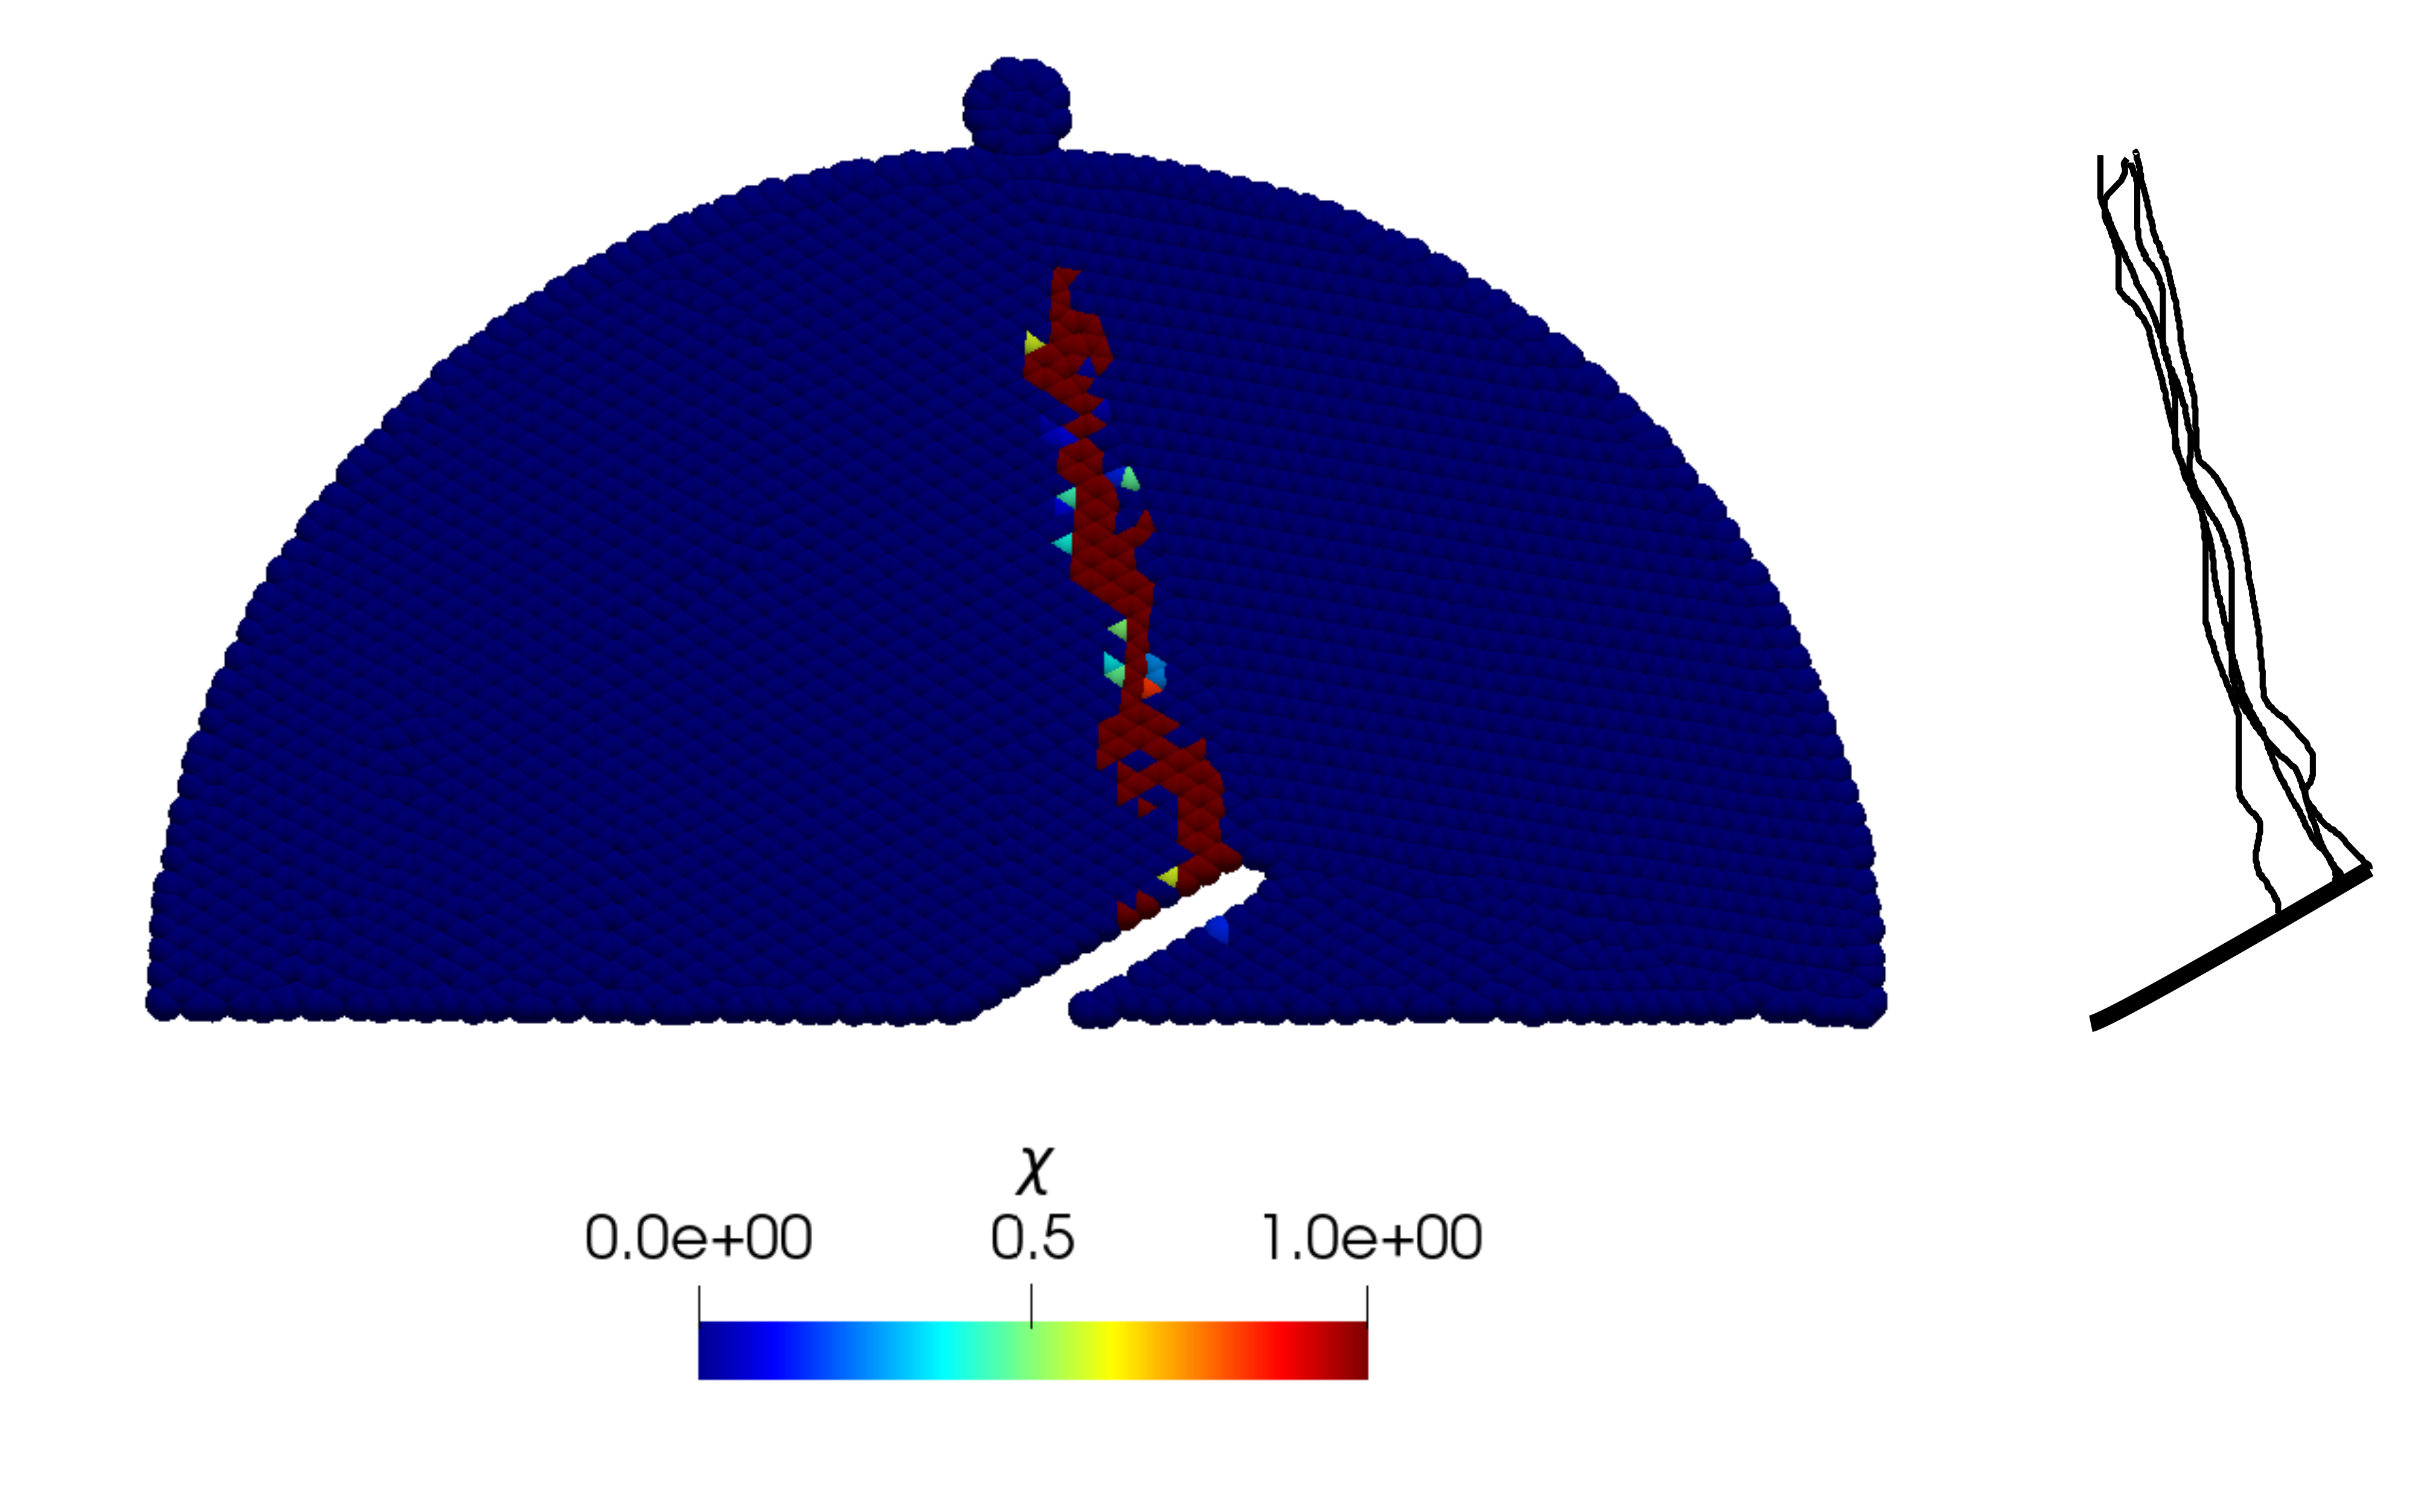
\includegraphics[width=0.49\textwidth]{./Figure-Angle-Forces-test-60-damage-pattern.png}}
\caption{Crack pattern for different notch inclination angle, and
  comparison with the experimental results  \cite{LIM_1993}.}
\label{fig:Figure-Angle-Forces-test-damage-pattern}
\end{figure}
%%%%%%%%%%%%%%%%%%%%%%%%%%%%%%%%%%%%%%%%%%%%%%%%%%%%%%%
Additionally, \ref{fig:plot-Angle-Forces-test} compare the peak load
between experiments and simulations for the notch inclination angles
0$^{\circ}$, 30$^{\circ}$ and 60$^{\circ}$. This figure proofs how the
eigensoftening-\acrshort{mpm} simulation can appropriately capture the
increasing trend of the peak load with the increasing notch angles in
the experiment.
%%%%%%%%%%%%%%%%%%%%%%%%%%%%%%%%%%%%%%%%%%%%%%%%%
\begin{figure}
  \centering
  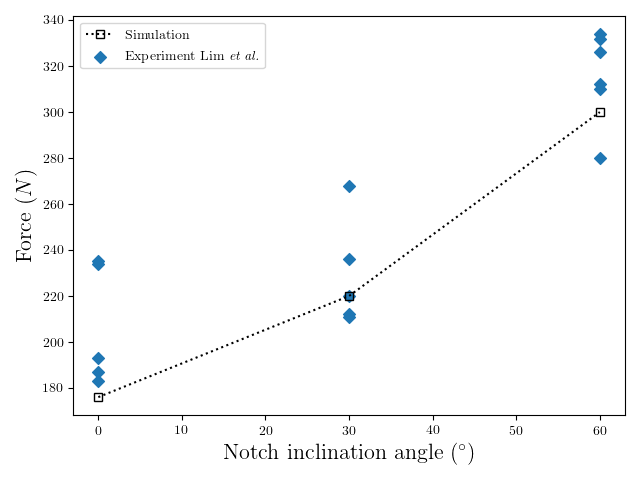
\includegraphics[width=0.7\textwidth]{./Figure-Angle-Forces-test}
  \caption{Numerical results compared with the experimental results \cite{LIM_1993}.}
  \label{fig:plot-Angle-Forces-test}
\end{figure}
%%%%%%%%%%%%%%%%%%%%%%%%%%%%%%%%%%%%%%%%%%%%%%%%%



\subsection{Drop-weight impact test}
\label{sec:3.3}
This section is devoted to proof
the accuracy of the eigensoftening algorithm within the \acrshort{mpm} framework when the behavior
of quasi-brittle materials under dynamic loading is simulated. One of the most interesting examples of this
loading case is the three-point bending test on a concrete notched beam when it is conducted under impact loading. Indeed, this experimental test is appropriate to be reproduced numerically with the explicit solver proposed in this paper since
fracture occurs in a period of milliseconds and waves propagate fast along the high strength
materials involved in the aforementioned test. Accordingly, small time steps are
required to achieve a numerically stable simulation.\\

An interesting case of this experimental test was reported by Zhang {\it et al.} \cite{Zhang_2009,Zhang_2010a}. As in the aforementioned study,
an impact hammer of 120.6 kg has been employed in the proposed simulations to drop it at an impact
speed of 2640 mm/s. The beam dimensions were 100 mm x 100 mm (B x D)
in cross section, and 420 mm in total lenght (L). The initial
notch-depth ratio was approximately 0.5, and the span, S, was fixed at
300 mm during the tests (see Figure
\ref{fig:geometry-drop-weight-impact-test}).
%%%%%%%%%%%%%%%%%%%%%%%%%%%%%%%%%%%%%%%%%%%%%%%%%%
\begin{figure}
  \centering
  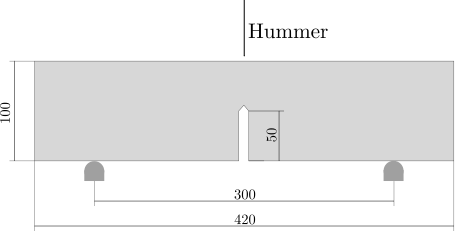
\includegraphics[width=0.8\textwidth]{./Figure-impact-test}
  \caption{Geometry and boundary condition of the drop-weight impact test.}
  \label{fig:geometry-drop-weight-impact-test}
\end{figure}
%%%%%%%%%%%%%%%%%%%%%%%%%%%%%%%%%%%%%%%%%%%%%%%%%%
The material adopted for the simulation was characterised by Navas
{\it et al.}~\cite{Navas_2017_ES}, being the material properties, such
as the material density, \gls{rho}, the compressive strenght, \gls{fc},
the tensile strenght \gls{ft}, the specific fracture energy, \gls{Gf},
and the elastic modulus \gls{E}, provided in table \ref{tab:concrete-properties}.\\
%%%%%%%%%%%%%%%%%%%%%%%%%%%%%%%%%%%%%%%%%%%%%%%%% 

\begin{table}
  \centering
  \begin{tabular}[]{c c c c c c c}
    \hline
      &   $\rho$   & $\text{f}_c$ & $\text{f}_t$ & $G_F$ &   E   & $\text{d}_{max}$ \\
      & (kg/m$^3$) &     (MPa)    &     (MPa)    & (N/m) & (GPa) & (mm) \\
    \hline
Value &    2368    &     102.7    &      5.4     &  141  &   31  &  12 \\
    \hline
  \end{tabular}
  \caption[Mechanical properties of thje concrete]{Mechanical
    properties of the high strenght concrete.}
  \label{tab:concrete-properties}
\end{table}
%%%%%%%%%%%%%%%%%%%%%%%%%%%%%%%%%%%%%%%%%%%%%%%%%
For the present research, a 2D setting of the experiment has been
adopted. Both the hammer and the concrete beam are explicitly
represented in order to properly capture the impact. Several levels of
discretisation were required to assess the objectiveness of the
obtained results. The results here exposed are from a discretisation
of 21576 material points and 3943 nodes. To achieve better results, an
unstructured grid layout has been adopted focusing the minimum nodal
spacing, 1.2 mm, in the middle of the beam and in the impact surface
of the hammer. For this simulation, \gls{gamma-lme} was fixed to
1.8, this low value of the regularization parameter smooth high stress
overshots after the impact. Here the stabilization properties of the \acrshort{lme}
described in \cite{Molinos2020} becomes crucial to achieve
non-spurious results. In fact, standard linear element were tested
with unsatisfactory results since grid-crossing occurs in the hammer
head producing non realistic forces.\\

First, the reaction and impact forces are validated against their
experimental counterparts. Since the impact forces applied by the
hammer and the reaction forces at the two supports were experimentally
measured, they are compared with numerical ones in Figure
\ref{fig:Reactions-Forces-impact-test}. 
%%%%%%%%%%%%%%%%%%%%%%%%%%%%%%%%%%%%%%%%%%%%%%%%%%%%%% 
\begin{figure}
  \centering
  \subfigure[Hammer forces]{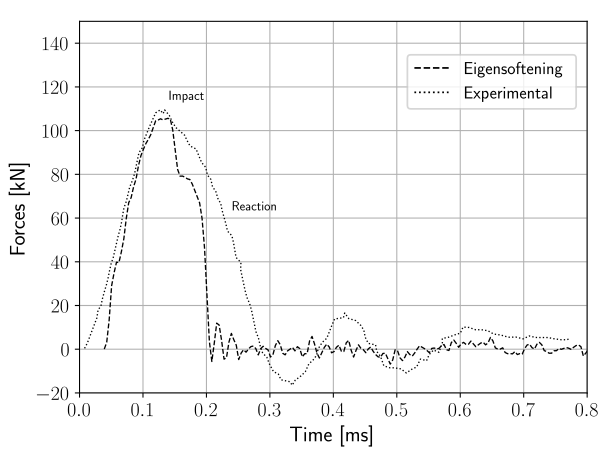
\includegraphics[width=0.8\textwidth]{Figure-impact-test-Forces-Time}}
  \subfigure[Reactions]{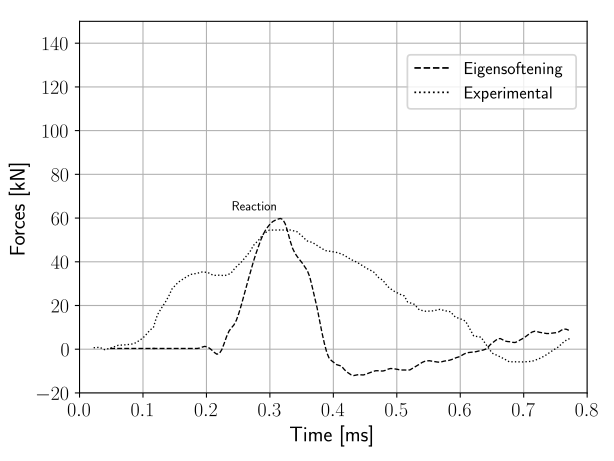
\includegraphics[width=0.8\textwidth]{Figure-impact-test-Reactions-Time}}
  \caption{Comparison of eigensoftening \textit{versus} experimental results.}
  \label{fig:Reactions-Forces-impact-test}
\end{figure}
%%%%%%%%%%%%%%%%%%%%%%%%%%%%%%%%%%%%%%%%%%%%%%%%%%%%%%
Note that the general trend of the impact forces was correctly
captured. Although the traditional \acrshort{mpm} implementation allows collision of two bodies, inaccurate energy conservation is obtained without the implementation of a conservative contact algorithm to reproduce the hammer impact in the beam.
Despite the observed discrepancies, this is out of the scope of this
document, although future research of authors will overcome this
limitation. Similarly, results of support forces will be more
realistic when modelled by a suitable contact algorithm instead of
avoiding any vertical displacement. Navas {\it et al.}
(2017)\cite{Navas_2017_ES} demonstrate the importance of the stiffness
of the support in order to obtain accurate results of the reaction
forces. Interesting contact algorithms within the \acrshort{mpm}
methodology are available in the literature
\cite{Bardenhagen_Contact_2001,XZhang_Contact_2011}.

Finally, longitudinal stress distribution and crack propagation are
depicted in Figure \ref{fig:Stress-vs-damage-impact-test}. Stress
evolution agrees with the results obtained by \cite{Navas_2017_ES}
under the \acrshort{otm} framework. Two additional considerations about
this results are concerning the interpolation technique. On the one hand,
in the opposite to the \acrshort{ugimp} shape function, \acrshort{lme}
allows unstructured grids. This is a remarkable benefit for this kind
of simulations since the majority of the computational effort is
clearly localised in a tiny region of the domain. On the other
hand, there is the possibility to reduce the shape function support to avoid
a material point in one side of the crack is affected by those in the
other side of the crack.
%%%%%%%%%%%%%%%%%%%%%%%%%%%%%%%%%%%%%%%%%%%%%%%%%%%%%%
\begin{figure}
\centering
\subfigure[t = 0.27 ms]{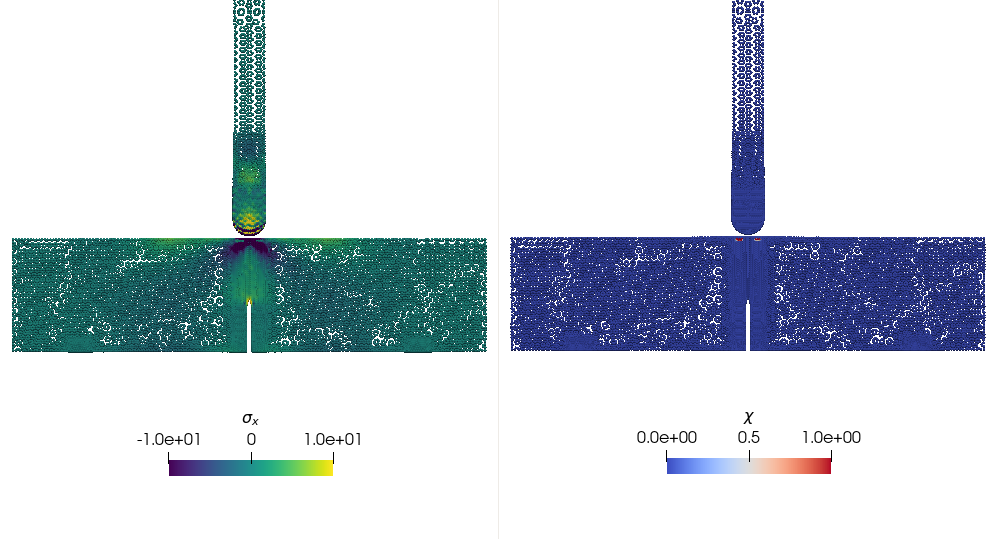
\includegraphics[width=0.83\textwidth]{./Figure-impact-test-Damage-vs-Stress-0005}}
\subfigure[t = 0.36 ms]{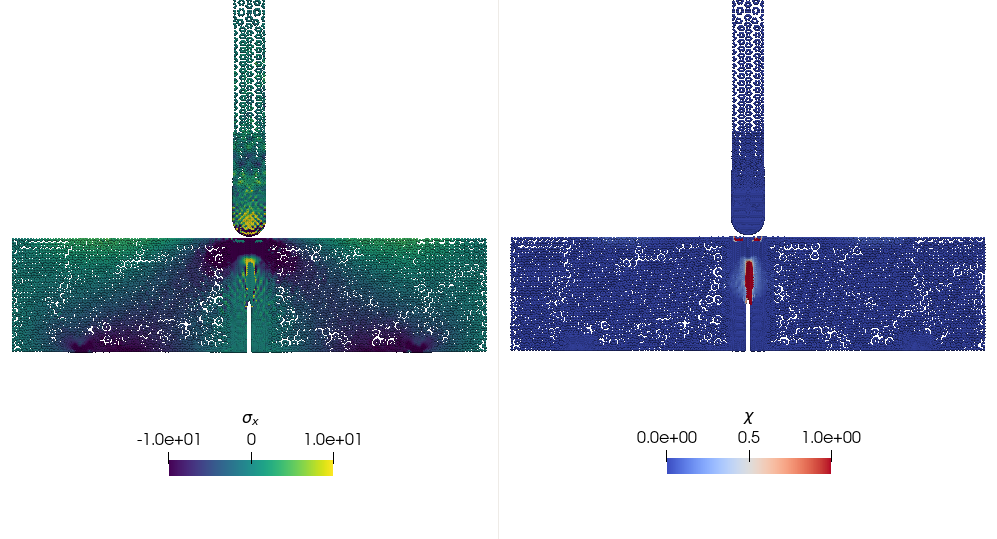
\includegraphics[width=0.83\textwidth]{./Figure-impact-test-Damage-vs-Stress-0015}}
\subfigure[t = 0.45 ms]{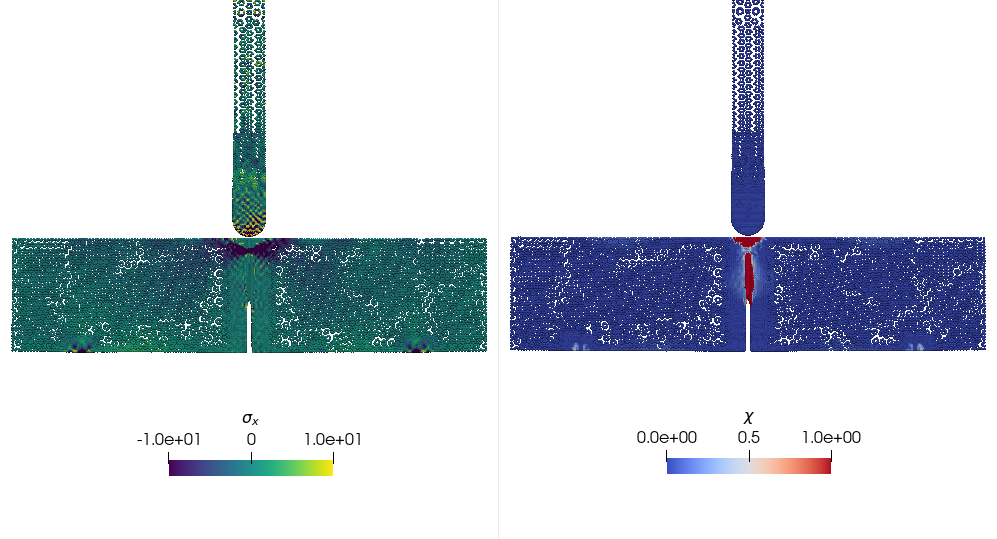
\includegraphics[width=0.83\textwidth]{./Figure-impact-test-Damage-vs-Stress-0030}}
\caption{Evolution of the stress tensor magnitude [MPa] for linear
  interpolation (pictures in the left side), and \acrshort{lme}
  (pictures in the right side). Both simulations performed with an
  eigenerosion algorithm.}
\label{fig:Stress-vs-damage-impact-test}
\end{figure}
%%%%%%%%%%%%%%%%%%%%%%%%%%%%%%%%%%%%%%%%%%%%%%%%%%%%%%

\section{Conclusions}
\label{sec:4}

The paper proposes the eigensoftening algorithm in a \acrshort{mpm} framework for quasi-brittle materials to overcome the limitations observed in the EigenMPM \cite{Zhang_EE_2020}. The overestimation of tensile 
stress and strain peaks in the fracture mechanism of quasi-brittle
materials and the stress oscillations observed with conventional
\acrshort{mpm} are faced. Based on the
EigenMPM approach to fracture, two additional improvements have been proposed in the present research in order to solve the shortcomings of the original concept pointed out in the aforementioned paper \cite{Zhang_EE_2020}.

Firstly, by introducing the concept of eigensoftening to the \acrshort{mpm} framework,
which allows to consider gradual failure process of each material point. This concept is analogous the softening law which is traditionally employed in the context
of cohesive fracture in \acrshort{fem}. Furthermore, this failure
criterion admits the design of more elaborated damage curves, which
can be employed in order to describe the failure process in more
sophisticated materials. Secondly to achieve better results, three new
numerical algorithms has been implemented. The \acrshort{lme}
approximants are employed to remove from
the solution those wiggles provoked by inaccuracies in the stress
integration and to avoid the ``tie-effect'' observed in the
\acrshort{ugimp}. The traditional time scheme of the \acrshort{mpm}
has been improved with a Newmark Predictor Corrector scheme as
well. And the traditional concept of element connectivity has been
removed to allow a more flexible and efficient implementation of
search algorithm. In this research, the aforementioned techniques have helped
to improve the results in fracture propagation through the
eigensoftening and eigenerosion algorithms.

Finally, further improvements of the present research are exposed. The
algorithm would have the ability to simulate of crack patterns in
composite material such as steel or carbon fiber reinforced
concretes\cite{Navas_2018_ES,Ruiz2019}. In addition, the eigensoftening
approach can be extrapolated to rock fracture in the same manner the
eigenerosion was~\cite{Wang2017}, taking into account that the
volumetric stiffness remains in order to support bulk loads. Also the
benefits of \acrshort{lme} can be exploited by adapting it through the
deformation gradient \cite{Kochmann2019}. \textit{A priori} this would
enhance the localisation properties of the proposed algorithms in more
sophisticated domains. And the implementation of a contact algorithm to model other impact cases such as bullets collisions. 

\section*{Acknowledgements}
The financial support to develop this research from the Ministerio de
Ciencia e Innovaci\'on, under Grant No. BIA-2016-76253 is greatly
appreciated. The first and the second authors also acknowledge the
fellowship Fundaci\'on Agust\'in de Betancourt and Juan de la Cierva
(FJCI-2017–31544) respectively.

\printglossaries

\appendix
%\addappheadtotoc
%\appendixpage
%\renewcommand{\theequation}{\Alph{section}.\arabic{equation}}

\section{Explicit Newmark Predictor-Corrector algorithm}
\label{sec:expl-pred-corr}
\begin{algorithm}[H]
  \DontPrintSemicolon
    %%%%%%%%%%%%%%%%%%%%%%%%%%%%%%%%%%%%%%%%%%%%%%%%%%%%%%%%%%%%%%%%%%%%%%%%%%%%%%%%%%%%%%
    \textbf{Update mass matrix :} $ \tens{m}_{I} = N_{Ip}^{k}\ m_p$ \;
    %%%%%%%%%%%%%%%%%%%%%%%%%%%%%%%%%%%%%%%%%%%%%%%%%%%%%%%%%%%%%%%%%%%%%%%%%%%%%%%%%%%%%% 
    \textbf{Explicit Newmark Predictor :}
    \begin{equation*}
      \vec{v}_I^{pred} = \frac{ N_{Ip}^{k} m_p (\vec{v}_p^k + (1 - \gamma)\ \Delta t\ \vec{a}_p^k)}{m_I}
    \end{equation*}\;
    %%%%%%%%%%%%%%%%%%%%%%%%%%%%%%%%%%%%%%%%%%%%%%%%%%%%%%%%%%%%%%%%%%%%%%%%%%%%%%%%%%%%%% 
    \textbf{Impose essential boundary conditions :} At the fixed
    boundary, set $\vec{v}_{I}^{pred} = 0$.\; 
    %%%%%%%%%%%%%%%%%%%%%%%%%%%%%%%%%%%%%%%%%%%%%%%%%%%%%%%%%%%%%%%%%%%%%%%%%%%%%%%%%%%%%% 
    \textbf{Deformation tensor increment calculation :}
    \begin{equation*}
      \Delta \tens{\varepsilon}_{p}^{k+1} = \Delta t\
        \dot{\tens{\varepsilon}_{p}}^{k+1} = \Delta t\ \left[ \vec{v}_{I}^{pred} \otimes
        \Grad{N_{Ip}^{k+1}} \right]^s
    \end{equation*} \;
    %%%%%%%%%%%%%%%%%%%%%%%%%%%%%%%%%%%%%%%%%%%%%%%%%%%%%%%%%%%%%%%%%%%%%%%%%%%%%%%%%%%%%% 
    \textbf{Update the density field :} $\rho_p^{k+1} =
    \frac{\rho_p^k}{1 + \mathit{tra}\left[\Delta\tens{\varepsilon}_{p}^{k+1}\right]}.$\;
    %%%%%%%%%%%%%%%%%%%%%%%%%%%%%%%%%%%%%%%%%%%%%%%%%%%%%%%%%%%%%%%%%%%%%%%%%%%%%%%%%%%%%% 
    \textbf{Compute stress field and update damage parameter}\;
    %%%%%%%%%%%%%%%%%%%%%%%%%%%%%%%%%%%%%%%%%%%%%%%%%%%%%%%%%%%%%%%%%%%%%%%%%%%%%%%%%%%%%% 
    \textbf{Balance of forces calculation :} Calculate the total grid
    nodal force $\vec{f}_{I}^{k+1} = \vec{f}_{I}^{int,k+1} + \vec{f}_{I}^{ext,k+1}$.\;
    %%%%%%%%%%%%%%%%%%%%%%%%%%%%%%%%%%%%%%%%%%%%%%%%%%%%%%%%%%%%%%%%%%%%%%%%%%%%%%%%%%%%%% 
    \textbf{Explicit Newmark Corrector :}
    \begin{equation*}
      \vec{v}_{I}^{k+1} = \vec{v}_{I}^{pred} + \gamma\ \Delta t\ \frac{\vec{f}_{I}^{k+1}}{\tens{m}_I^{k+1}}  
    \end{equation*}\;
    %%%%%%%%%%%%%%%%%%%%%%%%%%%%%%%%%%%%%%%%%%%%%%%%%%%%%%%%%%%%%%%%%%%%%%%%%%%%%%%%%%%%%%
    \textbf{Update particles lagrangian quantities :}
    \begin{align*}
      &\vec{a}_p^{k+1} = \frac{N_{Ip}^k\vec{f}_{I}^{k}}{\tens{m}_I^k}\\
      &\vec{v}_p^{k+1} = \vec{v}_p^n + \Delta t\
        \frac{N_{Ip}^k\
        \vec{f}_{I}^{k}}{\tens{m}_I^k}\\
      &\vec{x}_p^{k+1} = \vec{x}_p^n + \Delta t\
         N_{Ip}^k\ \vec{v}_{I}^{k} +
        \frac{1}{2}\Delta t^2\ \frac{N_{Ip}^k\
        \vec{f}_{I}^{k}}{\tens{m}_I^k}
    \end{align*}\;
    %%%%%%%%%%%%%%%%%%%%%%%%%%%%%%%%%%%%%%%%%%%%%%%%%%%%%%%%%%%%%%%%%%%%%%%%%%%%%%%%%%%%%% 
    \textbf{Reset nodal values}\;
    %%%%%%%%%%%%%%%%%%%%%%%%%%%%%%%%%%%%%%%%%%%%%%%%%%%%%%%%%%%%%%%%%%%%%%%%%%%%%%%%%%%%%% 
    \label{alg-epc}
    \caption{Explicit Newmark Predictor-Corrector scheme}
\end{algorithm} 

\section{Eigensoftening Algorithm}
\label{sec:eigens-algor-1}

\begin{algorithm}[H]
  \DontPrintSemicolon
  \KwInput{For each $p$, $\epsilon$-neighbourhood, $f_{t,p}$, $h_{\epsilon,p}$, $w_c$}
  \KwOutput{Return damage parameter $\chi = \{\chi_p\}$}
  % \KwData{Testing set $x$}
  $\chi_p \leftarrow \chi_p^{k}$ \;
  \For{$p$ to $N_p$}
  {
    \If{$\chi_p = 0$ \And $\epsilon_{f,p} = 0$}
    {
      \For{$q \in B_{\epsilon,p}$}
      {
        $\sigma_{q,I} \leftarrow \text{getEigenvaluesOf} (\sigma_{q}) $ \;
        \If{$\chi_q < 1$}
        {
          $ \sum m_p\sigma_{p,I} \leftarrow \sum m_p\sigma_{p,I} + m_q\sigma_{q,I}$ \;
        }
        $ m_p \leftarrow m_p + m_q$ \;
      }
      $\sigma_{p,\epsilon} \leftarrow \frac{1}{m_p} \sum m_p\sigma_{p,I}$\;
      \If{$\sigma_{p,\epsilon} > f_{t,p}$}
      {
        $\epsilon_{f,p} = \epsilon_{I,p}$ \;  
      }
      \ElseIf{$\chi_p \neq 1$ \And $\epsilon_{f,p} > 0$}
      {
        $\chi_p^{k+1} \leftarrow \min\Big \{1 , \max \{\chi_p^{k},
        \frac{(\epsilon_{I,p}- \epsilon_{f,p})\ h_{\epsilon,p}}{w_c}
        \} \Big \}$ \;
      }
    }
  }
    \label{alg-eigens}
    \caption{Compute damage parameter $\chi$}
\end{algorithm}

\section{Node-linked method for $\epsilon$-neighbourhood reconstruction}
\label{sec:node-linked-method-1}
\begin{algorithm}[H]
  \DontPrintSemicolon
  \KwInput{$I_0$ : Closest node for each particle}
  \KwInput{$I_{Nodes}$ : List of nodes close to each node}
  \KwInput{$Particles_I$ : List of particles close to each node}
  \KwOutput{$\text{neighbourhood}_{\epsilon}$ : $\epsilon$-neighbourhood for each particle}
  \For{$p$ to $N_p$}
  {
    For each $p$ get $I_0$\;
    Eval $I_{Nodes}(I_0)$ \;
    \For{$k \in I_{Nodes}(I_0)$}
    {
      $\text{neighbourhood}_{\epsilon}^{k+1}$ = $\text{neighbourhood}_{\epsilon}^{k} \cup Particles_I(k)$
    }
    \For{$p_{\epsilon} \in \text{neighbourhood}_{\epsilon}$}
    {
      \If{$distance(p_{\epsilon},p) > \epsilon $}
      {
        pop $p_{\epsilon}$ from neighborhood$_{\epsilon}$\;
      }      
    }
    
  }
  \label{alg-node-link}
  \caption{$\epsilon$-neighborhood reconstruction algorithm}
\end{algorithm} 

% name your BibTeX data base
\bibliography{Biblio} 

\end{document}


%%% Local Variables:
%%% ispell-local-dictionary: "en_GB"
%%% End:
